\documentclass[
    13pt, % Font size
    a4paper, % Paper format
    DIV14, % Margin calculation
    listof=totoc, % Include lists in TOC
    bibliography=totoc, % Include bibliography in TOC
    index=totoc, % Include index in TOC
    headsepline
]{scrreprt}


% Packages
\usepackage[english]{babel} % Language setting
\usepackage[utf8]{inputenc} % Input encoding
\usepackage[T1]{fontenc} % Font encoding
\usepackage{makeidx} % Index generation
\usepackage{url} % URLs
\usepackage{doc} % LaTeX symbols
\usepackage{graphicx} % Graphics
\usepackage{setspace} % Line spacing
\usepackage{float} % Improved figure positioning
\usepackage{geometry} % Page geometry
\usepackage{enumitem} % Enhanced lists
\usepackage{hyperref} % Hyperlinks
\usepackage{fancyhdr} % Custom headers and footers
\usepackage{booktabs} % Enhanced table aesthetics
\usepackage{multirow} % Multi-row tables
\usepackage{arydshln} % Dashed lines for tables
\usepackage{array} % Table customization
\usepackage{tabularx} % For automatic table column width
\usepackage{adjustbox} % For resizing tables
\usepackage{caption} % Custom table captions
\usepackage{xcolor} % Colors for table highlights
\usepackage{fontawesome} % Extra symbols (optional)
\usepackage[inline]{enumitem} % Provides inline enumerations

% Line spacing
\setstretch{1.3}

% Hyperref settings
\hypersetup{
    colorlinks=true,
    linkcolor=blue,
    filecolor=blue,
    urlcolor=blue,
    citecolor=blue
}

% Page geometry customization
\geometry{left=0.8in, right=0.8in, headheight=10pt, headsep=20pt, footskip=50pt}

% Header and footer settings
\pagestyle{fancy}
\fancyhf{} % Clear default header/footer
\fancyhead[R]{\textit{\leftmark}} % Chapter title on the right
\fancyfoot[C]{\thepage} % Page number at center

% Custom chapter/section titles
\renewcommand{\chaptermark}[1]{\markboth{#1}{}}
\renewcommand{\sectionmark}[1]{}

% Language selection command
\newcommand{\setlang}[1]{\selectlanguage{#1}\nonfrenchspacing}

% Add note about fallback font
% Fallback font information for environments without Calibri.
\newcommand{\fallbacknote}{\textit{Note: If Calibri is unavailable, the document defaults to Palatino font via mathpazo package.}}

\begin{document}


% TITLE PAGE:
\pagenumbering{roman}
\begin{titlepage}

\begin{center}

% University Title Section
\vspace*{2cm} % Adjust spacing at the top
\textbf{
\LARGE Ruprecht-Karls-Universität Heidelberg\\
\vspace*{0.5cm}
\smallskip
\Large Institute of Computer Science\\
\smallskip
\Large Heidelberg Institute for Geoinformation Technology\\
}

% Project Title Section
\vspace{2cm} % Add equal spacing between university title and project title
\textbf{\large Master's Thesis} % Studienarbeit, Interdisziplinaeres Projekt

\textbf{\LARGE
XGBoost-Based ML Framework for \\
\vspace{0.3cm}
Vandalism Detection in OpenStreetMap
}

% Student Details Section
\vspace{2cm} % Add equal spacing between title and details
{\large
\begin{tabular}{ll}
Name &:     Sri Pavan Sesha Sai Rallapalli\\
Matriculation number&: 4730140\\
Supervisor&:  Prof. Dr. Ullrich Köthe\\
Second Supervisor&: Prof. Dr. Alexander Zipf\\
Date of submission&:  31.01.2025
\end{tabular}
}

\end{center}

\end{titlepage}




% Empty page
\newpage
\thispagestyle{empty}
\null

% Acknowledgement
\newpage
\section*{\LARGE Acknowledgement}

I would like to express my deepest gratitude to my supervisors, Prof. Dr. Ullrich Köthe, Prof. Dr. Alexander Zipf, and Benjamin Herfort, for their invaluable guidance, expertise, and unwavering support throughout this thesis. Their constructive feedback and profound insights played a pivotal role in shaping the direction and outcome of my research.

Special thanks are extended to my colleagues and mentors at Heidelberg University, whose support and collaboration have significantly enriched my academic journey. I am particularly grateful to the Heidelberg Institute for Geoinformation Technology (HeiGIT) and the Computer Vision and Learning Lab (IWR) for providing essential resources and infrastructure, which were instrumental in the success of this work.

I am also deeply appreciative of the friendships and connections I have formed during my time as a master’s student. The support, motivation, and camaraderie shared with my peers have been a constant source of inspiration and strength.

Finally, I would like to express my heartfelt gratitude to my family for their unwavering love, patience, and encouragement throughout this journey. Your belief in me has been a cornerstone of my perseverance and success. This accomplishment would not have been possible without your enduring support.

\newpage
\section*{\LARGE Declaration of Independence}
I hereby certify that I have written the work myself and that I have not used any sources
or aids other than those specified and that I have marked what has been taken over from
other people’s works, either verbatim or in terms of content, as foreign. I also certify
that the electronic version of my thesis transmitted completely corresponds in content
and wording to the printed version. I agree that this electronic version is being checked
for plagiarism at the university using plagiarism software.

\vspace*{50pt}

\noindent
Sri Pavan Sesha Sai Rallapalli\\
Heidelberg, 31.01.2025

\newpage

\section*{\LARGE Summary}

OpenStreetMap (OSM) is one of the largest and most influential crowdsourced platforms for geospatial data. The collaborative nature of OSM allows individuals worldwide to contribute and update map data, providing a valuable resource for industries such as navigation, urban planning, disaster management, and environmental studies. However, this openness also makes OSM susceptible to vandalism—intentional or unintentional actions that degrade the quality and accuracy of its contributions. Detecting and mitigating vandalism is critical to maintaining the trustworthiness and utility of OSM data.

This thesis focuses on the development of a machine learning pipeline for detecting vandalism in both OSM contributions and changesets. Contributions represent individual edits to OpenStreetMap, which can include geographic features, metadata, relations, or other map-related elements, while changeset encapsulate a collection of related contributions submitted together in a single upload. The pipeline integrates data preprocessing, feature engineering, model training, evaluation, and visualization to deliver a robust solution that can operate at scale for both types of data. The overall objective is to create a system capable of accurately identifying vandalism while minimizing false positives and negatives, ensuring reliability in real-world applications.

\subsection*{Problem Statement}

The core challenge addressed in this thesis is the identification of vandalism within the vast and continuously evolving datasets of OpenStreetMap (OSM). Vandalism detection in OSM is a complex task due to several factors. Firstly, the scale of OSM contributions and changesets is immense, with millions of edits and changesets submitted monthly, making manual review infeasible. Secondly, vandalism manifests in diverse forms, including malicious edits, deliberate misinformation, and spurious changes, each requiring unique detection strategies. Some instances of vandalism are subtle and can closely resemble genuine edits, further complicating the detection process. Finally, ensuring data integrity in OSM often necessitates near real-time detection capabilities, especially in applications where timely and accurate geospatial data is critical. Addressing these challenges demands the development of an efficient and robust automated system capable of detecting vandalism with high precision and scalability.

\subsection*{Approach}

The research adopts a systematic approach to tackle the problem for both contributions and changesets, encompassing the following steps:

\noindent\textbf{Data Acquisition and Preparation:} Historical OSM contributions and changesets were curated into labeled datasets of vandalism and non-vandalism entries. These datasets serve as the foundation for model training and evaluation.

\noindent\textbf{Feature Engineering:} A diverse range of features was derived from raw data, capturing spatial, temporal, and user-specific characteristics for contributions and changesets. These features were carefully designed to maximize the model's ability to differentiate between vandalism and legitimate entries across both data types.

\noindent\textbf{Model Development and Training:} Two machine learning models were developed using the XGBoost algorithm, one for contributions and one for changesets. XGBoost was chosen for its efficiency, scalability, and ability to handle large datasets. Both models were trained on their respective labeled datasets to classify entries as vandalism or non-vandalism.

\noindent\textbf{Pipeline Design and Optimization:} The system was built as a modular pipeline capable of handling end-to-end processing, from raw data ingestion to prediction, for both contributions and changesets. Special attention was given to optimizing memory usage and computational efficiency, enabling the pipeline to process millions of entries in a scalable manner.

\noindent\textbf{Evaluation and Validation:} The models were rigorously evaluated using metrics such as accuracy, precision, recall, and F1-score. Separate test sets were designed to reflect real-world conditions for contributions and changesets, ensuring that the system performs well in production scenarios.

\noindent\textbf{Visualization and Insights:} The results were visualized through temporal and spatial analyses, including time-series graphs and heatmaps. These visualizations provide actionable insights into patterns of vandalism, such as geographic hotspots and temporal trends, for both contributions and changesets.

\subsection*{Results}

The developed system demonstrated strong performance, achieving high levels of accuracy and reliability for both contributions and changesets. Its ability to generalize across diverse test scenarios suggests that it is well-suited for real-world deployment. Visual analyses of the results highlighted meaningful trends in vandalism activity, enabling targeted interventions and enhanced monitoring by stakeholders.

\subsection*{Significance}

The contributions of this thesis extend beyond the technical development of vandalism detection systems for OSM contributions and changesets. By addressing the problem of data integrity in OSM, this work ensures that the platform can continue to serve as a reliable source of geospatial information. The methodology presented is not only applicable to OSM but also transferable to other crowdsourced systems facing similar challenges.

\subsection*{Future Directions}

While the current pipeline achieves high performance, there remain opportunities for further enhancement:

\noindent- Incorporating real-time processing to flag vandalism immediately after contributions or changesets are submitted.

\noindent- Investigating the use of deep learning for more nuanced detection of vandalism patterns.

\noindent- Developing community-driven tools that engage contributors in the validation and correction of flagged entries.

\subsection*{Conclusion}

This thesis presents a comprehensive and scalable solution to the problem of vandalism detection in OSM contributions and changesets. Through meticulous design and evaluation, the proposed system strikes a balance between accuracy, scalability, and usability. By ensuring data integrity, this work not only strengthens OSM as a platform but also supports the many industries and individuals that rely on its data.


\newpage
\section*{\LARGE Abstract}

OpenStreetMap (OSM) is a globally crowdsourced platform where volunteers can create and update geographic information. Although this open collaboration accelerates map growth and coverage, it also leaves OSM susceptible to vandalism—ranging from unintentional errors to deliberate malicious edits. Accurate and scalable vandalism detection mechanisms are therefore essential to maintain data quality and user trust.

This thesis presents a comprehensive machine learning pipeline for vandalism detection in OSM contributions and changesets, leveraging the XGBoost algorithm for classification. The pipeline is modular, encompassing data preprocessing, feature engineering, model training, and evaluation. Key features are extracted to capture spatial, temporal, and user-specific signals, enabling the model to distinguish subtle vandalism patterns from legitimate contributions. To reflect real-world deployment conditions, evaluation included test sets with realistic distributions of vandalism. Extensive experiments demonstrate the pipeline’s ability to achieve high accuracy, recall, and precision across diverse scenarios, with insights visualized through temporal and geographic analyses. The system is scalable, processing millions of entries efficiently, and adaptable, supporting both contribution- and changeset-level analyses.

This work advances the state of the art in vandalism detection by combining robustness, scalability, and actionable insights. This work represents a significant step toward ensuring data integrity in OSM by providing a efficient, and accurate vandalism detection system. Future research directions include the incorporation of real-time processing, deep learning techniques, and community-driven validation frameworks to further enhance vandalism detection and mitigation.

\newpage
\tableofcontents
\newpage

% Start Arabic numbering
\pagenumbering{arabic}
\setcounter{page}{1}

%-------------------------------------------------
% CHAPTER: INTRODUCTION
%-------------------------------------------------

\chapter{Introduction}\label{intro}

OpenStreetMap (OSM) \cite{osm_home} is a globally collaborative platform where volunteers contribute to creating and maintaining a free and openly accessible map of the world. It has experienced immense growth since its inception, fueled by a community of contributors who collectively add, edit, and curate geospatial information. Today, OSM data is extensively used in applications ranging from navigation and routing (e.g., in smartphone apps) to humanitarian and disaster response efforts. The open and inclusive nature of OSM enables anyone with internet access to contribute map data about roads, buildings, public facilities, and natural features. This diversity of inputs transforms OSM into a highly dynamic environment, ensuring that map information remains up-to-date and continuously expanding.

However, the very openness that drives OSM’s success also presents vulnerabilities. One of the most pressing challenges is vandalism \cite{vandalism_osm}—the deliberate or accidental submission of erroneous or malicious edits that can undermine data integrity and trust. Vandalism can appear in countless forms: from adding fictitious roads that do not exist on the ground, to completely removing landmarks critical to local navigation. While some vandalism is benign or arises from well-meaning but inexperienced contributors, other acts can be maliciously intended to mislead or disrupt the platform. Beyond obvious malicious acts, subtler forms of vandalism can also have significant repercussions on OSM’s quality. For instance, an experienced vandal could modify map geometry slightly or alter textual metadata in ways that go unnoticed by human reviewers for extended periods.

Given that OSM is utilized globally by a vast ecosystem of researchers, developers, corporations, and governmental agencies, maintaining high data quality is of paramount importance. Public and private sectors rely on OSM for tasks ranging from route planning to epidemiological studies. Errors injected by vandalism risk damaging user confidence and may have real-world consequences, especially in critical situations such as emergency response. Manual review processes, while helpful, cannot keep pace with the enormous inflow of daily edits, which numbers in the millions. As a result, automated techniques—particularly those rooted in machine learning (ML)—are increasingly integral to the ongoing stewardship of OSM data.

\section{Motivation and Significance}
\label{sec:motivation_significance}

The motivation behind this thesis stems from the widespread and escalating demand for accurate, timely identification of harmful OSM edits. Early detection of vandalism is crucial for preventing the proliferation of erroneous information across the numerous services and applications that depend on OSM data. Once inaccurate edits propagate into navigation software or analytics tools, they can create cascading effects, such as misrouting, resource misallocation, or even compromised safety in critical operations. By catching and rectifying vandalism early in the data pipeline, the reliability of OSM can be greatly enhanced. Automated detection methods provide a compelling solution. They can continuously analyze large volumes of OSM edits in near real-time, generating alerts for human moderators. Modern machine learning techniques—especially ensemble-based algorithms like XGBoost \cite{xgboost_documentation, xgboost_paper}—are well-suited to handling structured data at scale. These methods can parse complex interactions among features, ranging from contributor histories to geometric attributes of map features, to identify suspicious patterns. When designed efficiently, ML-driven systems complement the volunteer OSM community, creating a more robust and resilient mapping infrastructure.

A prime example of institutional commitment to OSM data quality is the Heidelberg Institute for Geoinformation Technology (HeiGIT)\cite{heigit_website}, which focuses on developing advanced geoinformation services and open-source solutions. Many of HeiGIT’s tools and research initiatives revolve around OSM, including the analysis of changesets for data quality. However, existing methods primarily target vandalism detection at the changeset level \cite{Li2021, Yuan2022}—i.e., examining entire upload sessions in one batch. While changeset-based detection is vital, it may overlook granular anomalies that appear in \emph{individual} contributions. Contributions represent single edits to OpenStreetMap data, encompassing the addition or modification of geographic features, metadata, relations, or other map-related elements. By contrast, \emph{changesets} \cite{osm_changesets} encapsulate multiple contributions grouped together in a single upload. Although some prior studies have outlined changeset-level strategies, there is a noticeable gap in comprehensive \emph{contribution-level} vandalism detection.

Addressing this gap forms a central goal of the present work. This thesis proposes a dual-focus pipeline—one that handles detection for contributions while still supporting the changeset-level perspective—to ensure that both large-scale and fine-grained vandalism patterns are identified. By bridging these two granularities, the system aims to catch subtle edits that might slip under changeset-level scrutiny, as well as wider malicious behavior affecting multiple map features within a single session. In doing so, the approach aspires to bolster OSM data integrity for crucial real-world applications, from advanced routing systems to crisis management tasks, where the accuracy of map data can be a decisive factor in outcomes.


\section{Overview of the Research Problem}
\label{sec:overview_problem}

Malicious edits in OSM may be intentionally disruptive (e.g., deleting large swaths of roads) or subtly misleading (e.g., altering a place name by a small but impactful degree), whereas unintentional errors arise from well-meaning contributors with limited expertise. This wide spectrum of vandalism types, compounded by OSM’s global scale, makes automated detection both crucial and difficult. Several factors underscore the complexity of vandalism detection. First, the volume of OSM edits is immense, with millions of contributions and changesets generated monthly. Attempting to monitor such a continuous torrent of data manually or using naive methods is infeasible. Second, vandalism can materialize in diverse ways: from single-tag manipulation to multi-faceted changeset alterations. Generic heuristic-based rules often fail to capture novel or evolving attack patterns, especially those that mimic legitimate modifications.

From a computational standpoint, traditional techniques that scan the dataset in a single pass tend to become intractable at scales involving hundreds of millions of records. Efficient chunk-based processing, with parallelized feature extraction and classification, is essential for real-time or near real-time decision-making. A robust system must therefore balance high accuracy with performance requirements. If the approach becomes too slow or resource-intensive, it risks impracticality in real-world deployment scenarios where OSM data are continuously updated across diverse global regions.

In summary, the research problem centers on designing an automated, scalable framework capable of identifying a multitude of vandalism types in OSM’s ever-growing data. Such a system should handle both fine-grained edits at the \emph{contribution} level and larger-scale patterns discernible at the \emph{changeset} level, bridging the gap between localized anomalies and session-wide disruptions.

\section{Scope of the Thesis}
\label{sec:thesis_scope}

This thesis tackles the specific task of building and evaluating a scalable machine learning pipeline for vandalism detection in OSM, addressing both \emph{contribution-level} and \emph{changeset-level} analyses. While the broader realm of OSM data quality includes numerous challenges (e.g., incomplete tagging, schema inconsistencies, or map validation), this work focuses on malicious or unintentional edits that significantly degrade spatial or attribute integrity. Within this defined scope, the thesis encompasses four main areas of investigation:
\begin{itemize}
    \item \textbf{Feature Engineering:} Identify and extract diverse features spanning \emph{geometric}, \emph{textual}, \emph{user-history}, \emph{temporal}, \emph{spatial}, \emph{map-based}, and \emph{OSM element–focused} domains. These include bounding-box changes, tag modifications, user edit frequencies, time-of-day patterns, map feature indicators (e.g., roads, buildings), and historical context of edited objects. Such a rich feature set ensures that the model can detect vandalism signals at multiple levels of granularity, from small metadata changes to large-scale deletions.
    \item \textbf{Pipeline Architecture:} Devise a robust, end-to-end workflow capable of handling massive OSM datasets through chunk-based data loading and parallelized feature extraction. The architecture should accommodate both contribution-level and changeset-level data, ensuring that it can process large volumes of edits in a scalable manner. Techniques such as distributed model inference and memory-efficient data handling are employed to sustain high throughput without sacrificing predictive accuracy.
    \item \textbf{Model Training and Evaluation:} Develop and train an XGBoost classifier (or related ensemble methods), experimenting with hyperparameter tuning to optimize performance. The pipeline is validated against labeled data (contribution-level and changeset-level) for training and validation, while also facilitating large-scale inference on unlabeled data. Metrics of interest include precision, recall, F1-score, and computational efficiency, with a focus on achieving balanced performance suitable for real-time or near real-time vandalism detection.
    \item \textbf{Performance Assessment:} Conduct comprehensive benchmarks to compare accuracy and resource usage in various scenarios. Special attention is given to user-history signals and contextual features that can influence detection performance, along with analyzing how chunk-based processing affects throughput. The evaluation explores whether the pipeline can effectively detect subtle single-edit vandalism and more obvious multi-edit disruptions at the changeset level.
\end{itemize}

By restricting the thesis to these focal points, the research provides a specialized yet adaptable framework that can be integrated into existing OSM oversight tools. The methodology does not address every nuance of OSM data quality—such as complex semantic tagging validation or duplication detection—but instead aims to produce a high-impact solution for automated vandalism identification. Ultimately, the combination of detailed feature engineering, a scalable pipeline, and a tailored ML model positions this thesis to offer tangible advancements in OSM data integrity for real-world scenarios.


\section{Objectives and Research Questions}

The overarching aim of this thesis is to develop a robust and scalable machine learning framework for detecting vandalism in OpenStreetMap (OSM) contributions and changesets. The objectives of the research are as follows:

\begin{itemize}
  \item To develop a comprehensive set of features capturing spatial, temporal, textual, and user-specific signals indicative of vandalism. This involves leveraging diverse data characteristics to enhance the model’s ability to distinguish between legitimate contributions and malicious edits.

  \item To design and implement a highly scalable machine learning pipeline capable of handling the extensive volume of OSM data with minimal memory overhead. Computational efficiency is a critical requirement for processing millions of contributions generated monthly.

  \item To achieve high predictive performance, measured through accuracy, precision, and recall, while minimizing false positives that could overwhelm human reviewers. The solution must strike a balance between predictive power and practical usability.

  \item  To investigate the role of historical features, user editing behavior, and other contextual cues in improving vandalism detection. This includes exploring the contributions of these features to overall model performance under various real-world scenarios.
\end{itemize}

\subsection*{Research Questions}

This thesis addresses key challenges associated with vandalism detection in OSM, framed around themes such as feature effectiveness, scalability, performance trade-offs, and real-world integration. It investigates which features are most effective in distinguishing vandalism from legitimate contributions, explores methods for processing large-scale datasets efficiently, and evaluates the trade-offs between model complexity and usability in real-world deployments. Additionally, it considers how the proposed solution can be seamlessly integrated into existing OSM workflows while maintaining high detection accuracy and operational feasibility.

\vspace*{1cm}
\noindent By focusing on these core aspects, the thesis ensures a comprehensive exploration of both technical and practical dimensions of vandalism detection, advancing the understanding of this critical problem and offering a robust framework for its solution.


\section{Thesis Outline}

To comprehensively address these questions, the thesis is organized into multiple chapters:

\begin{itemize}
  \item \textbf{Chapter \ref{intro}: Introduction} – Provides an overview of the OSM vandalism problem, the motivation for ML-based detection, and the core objectives of this thesis.
  \item \textbf{Chapter \ref{background}: Background and Related Work} – Discusses past and contemporary approaches to OSM vandalism detection, including rule-based and machine learning methods. Also reviews common challenges and feature engineering practices.
  \item \textbf{Chapter \ref{methods}: Methodology} – Outlines the method used in building the ML pipeline, detailing data preprocessing, feature design, hyperparameter tuning, and the step-by-step architecture of the solution.
  \item \textbf{Chapter \ref{evaluation}: Evaluation} – Describes the experiments conducted to assess model accuracy, scalability, and robustness. Includes comparative analyses with baseline methods and exploration of feature ablation studies.
  \item \textbf{Chapter \ref{conclusion}: Conclusion and Future Work} – Summarizes the main findings, emphasizes contributions, and proposes directions for future research and enhancements.
\end{itemize}

By systematically exploring these chapters, readers will gain both theoretical and practical insights into how machine learning can effectively combat vandalism in large, dynamic geospatial datasets such as OpenStreetMap.

%-------------------------------------------------
% CHAPTER: Background and Related Work
%-------------------------------------------------

\chapter{Background and Related Work}\label{background}

OpenStreetMap (OSM) has evolved from a modest, community-driven project into a globally influential mapping platform, hosting millions of user contributions each month. This section offers a comprehensive overview of vandalism detection research within OSM and analogous collaborative platforms, highlighting the transition from basic rule-based solutions to sophisticated machine learning (ML) methods. It also presents a comparative analysis of state-of-the-art models for tabular data (XGBoost, TabNet, FT-Transformers), along with an examination of the challenges in effectively scaling these solutions.

\section{Introduction to Vandalism Detection in Collaborative Platforms}

Vandalism—intentional or harmful edits that degrade the integrity of shared data—poses a recurring challenge across various crowdsourced systems. In these environments, anyone can modify or add content, creating a tension between openness and quality control \cite{Adler2010, Heindorf2017, MartinezRico2019}. Early detection of vandalism is paramount: spurious or malicious edits can undermine user trust and lead to real-world consequences, particularly when erroneous map information propagates into critical domains such as navigation or disaster management. The next sections focus on OSM-specific methods but also draw parallels from other platforms to emphasize recurring themes in vandalism research.

Vandalism is not exclusive to OSM. Wikipedia and Wikidata face similar challenges: open-edit models yield high coverage but invite malicious contributions. Adler et al. (2010) introduced WikiTrust to detect vandalism in Wikipedia, evaluating editor reputation and content revisions \cite{Adler2010}. Heindorf et al. (2017) extended this logic to Wikidata using Random Forest classifiers enriched with metadata cues \cite{Heindorf2017}. Publicly available vandalism corpora—like WDVC-2015—fostered large-scale supervised learning, while deep learning approaches (e.g., Martinez-Rico et al. (2019) \cite{MartinezRico2019}) showcased improvements in capturing textual nuances. These cross-platform studies highlight a shared need for reliable labeling, scalable architectures, and robust retraining strategies in the face of evolving vandalism.

\section{Evolution of Vandalism Detection in OSM}
\label{sec:evolution_osm_vandalism}

\subsection{Early Manual and Heuristic Defenses}
In OSM’s early phases, community members monitored edits manually—relying on mailing lists, discussion forums, and direct communication to identify suspect contributions. However, as the contributor base grew, it became clear that manual checks alone could not keep pace with the rapid influx of edits. Heuristic-based tools soon emerged, such as OSMPatrol and OSMCha, each flagging large bounding-box expansions or mass deletions for closer inspection \cite{OSMPatrol, OSMCha, Neis2012}. These systems proved adept at catching conspicuous vandalism but showed limited adaptability. Rules set for bounding-box changes, for instance, triggered many false positives (legitimate large edits) and failed to detect subtle manipulations. Community volunteers recognized the need for more flexible, data-driven approaches.

\subsection{Clustering and Hybrid Approaches}
While supervised methods brought significant improvements, some efforts explored clustering or hybrid techniques to detect anomalies. Truong et al. (2018) clustered edits with similar spatial or metadata profiles, identifying suspicious outliers \cite{Truong2018}. In a follow-up study, Truong et al. (2020) created OSMWatchman, a Random Forest classifier that combined user statistics, changeset metadata, and spatial context to detect vandalized contributions \cite{Truong2020}. Despite better performance, these studies revealed the persistent challenge of limited labeled data for real-world validation, motivating further exploration of advanced machine learning models capable of handling diverse OSM features.

\subsection{Transition to Machine Learning}

To overcome the static nature of heuristics, researchers introduced supervised ML models that leveraged labeled vandalism corpora. Such models integrated various features—edit size, changeset text, user reputation—to classify suspicious edits. Li et al. (2021) demonstrated the efficacy of incorporating user-behavior embeddings alongside content-based features, improving precision and recall over heuristic baselines \cite{Li2021}. Similarly, Yuan et al. (2022) utilized an attention-based neural architecture to handle intricate textual and geometric relationships within changesets \cite{Yuan2022}. These works underscored the adaptability and scalability of ML-driven frameworks, paving the way for more advanced or hybrid approaches in OSM vandalism detection.

These embedding-based and attention-driven methods represent advanced machine learning approaches for vandalism detection, each addressing unique aspects of OpenStreetMap (OSM) data analysis while sharing common limitations.

\textbf{Embedding-Based Methods:}
Embedding-based methods, as demonstrated by Li et al. (2021), focus on representing user behaviors through dense vector embeddings. By analyzing historical data such as contribution frequency, geographic focus, and tagging patterns, embeddings capture nuanced behavioral traits indicative of malicious edits. These representations are then incorporated into Gradient Boosted Decision Trees (GBDT) to enhance detection performance. While this approach significantly boosts recall and precision compared to traditional methods, it comes with notable challenges. Embedding-based systems require extensive historical data, excluding new or low-activity users, and their computational demands for embedding generation and maintenance can complicate real-time or large-scale deployment.

\textbf{Attention-Based Methods:}
Attention-based methods take a different approach by leveraging deep learning architectures to dynamically focus on the most relevant aspects of changeset data. Yuan et al. (2022) proposed a multi-head attention mechanism that prioritizes important features within changeset metadata, textual attributes, and geometric deltas. This allows the model to effectively process intricate relationships in the data, achieving high accuracy in detecting complex vandalism patterns. However, this method’s reliance on large labeled datasets and considerable GPU resources presents practical limitations, particularly in settings with limited computational capacity or scarce labeled data.

\textbf{Comparative Analysis:}
Despite their methodological differences, both embedding-based and attention-driven approaches share common strengths and challenges. They emphasize the importance of user-centric signals, geometry modifications, and textual cues in vandalism detection. However, obstacles such as limited labeled data, high computational costs, and the dynamic nature of vandalism patterns persist. These challenges underline the need for scalable and efficient solutions that balance performance with operational feasibility.

\section{Comparison of ML Models for Tabular OSM Data}
\label{sec:ml_comparison_for_osm}

While OSM data may appear heterogeneous—encompassing geometric, textual, temporal, and user-centric attributes—it often ultimately resides in tabular form. For such structured data, three notable machine learning models warrant detailed consideration: XGBoost, TabNet, and FT-Transformers.

\subsection{XGBoost: Extreme Gradient Boosting}
XGBoost is a gradient-boosted decision tree (GBDT) model recognized for its high performance and computational efficiency \cite{xgboost_paper}. By constructing multiple decision trees and optimizing their combination through gradient boosting, XGBoost produces robust predictions for binary classification tasks such as vandalism detection in OSM \cite{Chen2016}. The model excels in adaptability, effectively handling mixed data types, including numerical and categorical features. This makes it particularly suitable for OSM data, which integrates diverse attributes such as changeset metadata, user behavior metrics, and geometric properties. Additionally, XGBoost is computationally efficient, offering fast training and inference times, and its feature importance rankings provide interpretability, allowing insights into the most predictive attributes. Its scalability is another advantage, supporting parallel computation to handle large datasets efficiently. However, XGBoost does have limitations: it heavily relies on well-engineered features, requiring significant preprocessing and domain knowledge, and it may struggle with extremely high-dimensional or sparse data compared to deep learning models like FT-Transformers.

\subsection{TabNet: A Deep Learning Model for Tabular Data}
TabNet, a neural network explicitly designed for tabular data, leverages an attention mechanism to dynamically focus on the most relevant features during training \cite{Arik2021}. This feature reduces the need for extensive feature engineering while retaining interpretability through sparse attention mechanisms that highlight feature importance for individual predictions. Additionally, TabNet is adept at handling hierarchical feature dependencies, uncovering intricate relationships in data. Despite these strengths, TabNet requires longer training times compared to XGBoost, especially for smaller datasets, and performs best on larger datasets where its capacity is fully utilized. Its higher computational resource demands during both training and inference further limit its practicality for medium-sized datasets like those in OSM.

\subsection{FT-Transformers: Transformer Models for Tabular Data}
FT-Transformers extend the transformer architecture, originally designed for natural language processing (NLP), to tabular data by tokenizing features and employing self-attention mechanisms \cite{Gorishniy2021}. These models excel in capturing complex feature interactions across high-dimensional or sparse datasets, reducing dependence on manual feature engineering. FT-Transformers are particularly well-suited for datasets with intricate relationships between features, enabling end-to-end learning. However, these models are computationally intensive, with significant resource requirements for training and inference. Additionally, as a relatively new approach, FT-Transformers lack the mature tooling and documentation available for XGBoost. For smaller datasets, their performance improvements often do not justify the added complexity, making them less appealing for tasks such as OSM vandalism detection.

\subsection{Model Selection: Why XGBoost?}
In the context of vandalism detection, XGBoost emerges as the most suitable model for OSM data due to its balance of accuracy, interpretability, and computational efficiency. Studies have demonstrated that XGBoost consistently matches or outperforms deep learning–based models like TabNet or FT-Transformers for structured datasets \cite{Chen2016, Gorishniy2021}. Its ability to adapt to diverse feature types and provide interpretable feature importance rankings aligns well with the requirements of detecting vandalism in OSM. Moreover, the computational efficiency of XGBoost, makes it a practical choice for real-world implementation. As a result, the pipeline proposed in this thesis incorporates XGBoost to accommodate the diverse attributes of OSM edits effectively.


\section{Current Challenges in Vandalism Detection Research}

Despite progress, OSM vandalism detection still faces key hurdles:

\noindent
\textbf{Label Scarcity and Quality.}
High-quality labeled datasets for vandalism remain limited. Studies like Li et al. (2021) \cite{Li2021} introduce corpora, but these are not always updated or comprehensive, restricting the model’s ability to adapt to evolving malicious behaviors. Crowdsourced labeling or semi-supervised learning could partially alleviate this shortfall.

\noindent
\textbf{Scalability Demands.}
Given OSM’s rapid editing pace, handling potentially millions of updates daily can overburden even sophisticated ML systems. Efficient data chunking, parallel processing, and incremental model updates are required, as highlighted by Yuan et al. (2022) \cite{Yuan2022}, to keep pace with near real-time ingestion.

\noindent
\textbf{Adaptability to Evolving Vandalism.}
Attack vectors change over time, whether through new editing tools or emergent malicious patterns. ML solutions must be retrained periodically on fresh data, or employ online learning approaches, to remain robust against newly crafted disruptions.


\section{Summary}

In summary, OSM vandalism detection has transitioned from simple rule-based alerts to data-intensive, ML-based solutions. Key insights from Wikidata and Wikipedia underscore the broad utility of supervised learning for collaborative platform vandalism, while embedding-based and attention-driven methods exemplify cutting-edge OSM research. However, large-scale deployments require trade-offs in model selection, leaning toward robust yet efficient algorithms like XGBoost, and well-crafted features spanning textual, geometric, user-centric, temporal, and additional map-based domains.

This thesis builds on the strengths of these approaches by adopting a balanced strategy. Specifically, it leverages rich features from OSM data and integrates them into scalable tree-based machine learning models, such as XGBoost. This approach aims to combine the interpretability and efficiency of traditional models with the robustness of feature-rich representations, thereby addressing the practical limitations identified in embedding-based and attention-driven methods.

The next chapters detail how this thesis builds upon these findings to propose an XGBoost-driven pipeline, balancing performance and scalability in detecting malicious edits across OSM contributions and changesets.


%---------------------------------------------
% Chapter 3: Methods
%---------------------------------------------
\chapter{Methods}
\label{chap:methods}

\noindent
This chapter presents the methodological framework designed to detect vandalism across OpenStreetMap (OSM) contributions. Building on the insights from the background chapter (Chapter~\ref{background}), the methodology addresses two core demands of OSM data: handling its substantial volume and diversity, and capturing the multitude of vandalism patterns that may arise in small, individual edits or large, session-wide changes. The approach hinges on a configurable pipeline that can be executed independently on \textbf{contribution-level} data (fine-grained edits) or \textbf{changeset-level} data (aggregated sessions). By retaining a similar structure but separate executions for each perspective, the pipeline captures unique signals essential for robust vandalism detection without conflating their distinct data structures.

\section{Introduction to the Methodology}
\label{sec:introduction_methods}

The central challenge in OSM vandalism detection is twofold:
\begin{enumerate}[label=(\arabic*)]
    \item effectively managing a high-throughput data stream (often tens of millions of edits each month), and
    \item accurately detecting a broad spectrum of malicious behaviors, ranging from subtle, localized edits to extensive, orchestrated attacks within a single changeset session.
\end{enumerate}

In response, the proposed pipeline unites parallel processes for contribution-level data and changeset-level data, powered by a core machine learning workflow centered on \textbf{XGBoost}. Drawing on chunk-based feature extraction, hyperparameter optimization, and rigorous evaluation strategies, this chapter demonstrates how the pipeline copes with OSM’s dynamic nature while retaining interpretability and efficiency. Furthermore, it covers strategies to enhance changeset-level detection using insights from contribution-level predictions, ensuring minimal gaps in coverage.

\subsection{Purpose and Goals}
\label{sec:purpose_and_goals}

The overarching purpose of this methods chapter is to detail how the framework confronts OSM’s colossal data scale and diverse vandalism patterns. Specifically, the key objectives include:

\begin{itemize}
    \item \textbf{High-Volume Data Throughput}:
    Designing a chunk-based pipeline to process millions of monthly edits within hours, keeping computational and memory overhead in check.
    \item \textbf{Dual Data Perspectives}:
    Facilitating separate pipeline executions for \emph{contribution-level} (isolated edits) and \emph{changeset-level} (session-wide batches), allowing each vantage to expose particular vandalism indicators.
    \item \textbf{Core Classification Model (XGBoost)}:
    Exploiting XGBoost’s capability to handle structured tabular data with high accuracy and interpretability. Hyperparameter tuning is incorporated to optimize predictive performance.
    \item \textbf{Ensuring Strong Predictive Metrics}:
    Maintaining precision, recall, F1-score, AUC-PR, and ROC-AUC at levels sufficient to minimize both missed vandalism and false alarms.
    \item \textbf{Real-Time or Near Real-Time Feasibility}:
    Achieving inference speeds that suit short-window detection (e.g., every 5 minutes) and large-file batch processing (monthly updates in 1--2 hours). This aligns with OSM’s evolving data streams and the operational needs of platforms like HeiGIT.
    \item \textbf{Feature Diversity and Scalability}:
    Unifying user behaviors, OSM element metadata, temporal and geometric signals, and textual attributes, all in a scalable manner to detect subtle or overt malicious edits.
    \item \textbf{Enhancing Changeset-Level Detection with Per-Edit Insights}:
    Integrating aggregated per-contribution predictions (hyper-classifier) and fusing them with a normal changeset model (meta-classifier) when needed, improving session-wide detection of mass or systematic vandalism.
\end{itemize}

In meeting these goals, the pipeline provides a holistic solution that pinpoints vandalism early—protecting OSM’s data integrity and mitigating the broader risks of malicious edits in downstream applications such as navigation or disaster response.

\subsection{Data Perspectives}
\label{sec:data_perspectives}

\noindent
One of the most distinctive aspects of our methodology is the deliberate treatment of OSM data
at two complementary levels: contribution-level and changeset-level. In many crowdsourced
environments, including OSM, the simplest unit of data is often an individual edit or contribution—such as adding a building tag or updating a highway’s geometry. However, edits in OSM
are commonly submitted in groups known as changesets, each of which may contain numerous
contributions made during a single upload session. Vandalism can thus occur in subtle, isolated
edits or in large clusters of malicious activity spanning many map elements. Although the pipeline remains consistent in structure, it can be run independently on two data perspectives, each addressing different vandalism scenarios:

\paragraph{Contribution-Level Data.}
Within this perspective, each record corresponds to a single updated feature, such as a node or way. By analyzing contributions at this level, the system can detect localized anomalies—an abrupt coordinate shift, the removal of a crucial tag, or the introduction of nonsensical text. This fine-grained view is essential because vandalism often arises in small but impactful edits. A single outlier edit could relocate a landmark inappropriately, or rename a  well-known city with offensive text, and it is the contribution-level analysis that is best poised to flag such granular behavior.

\paragraph{Changeset-Level Data.}
While the contribution-level approach captures fine detail,
a supplementary view emerges when edits are grouped by the changeset in which they were
committed. In this changeset-level perspective, the entire batch of edits made by a user during
one editing session is evaluated collectively. This viewpoint is valuable because it can detect
broad or systematic attacks—for example, a user who deletes hundreds of roads across disparate
locations in one changeset. Even if individual edits look innocuous by themselves, the aggregate
pattern might reveal extensive vandalism. By examining changeset-wide metrics like the ratio
of deleted features, the number of continents affected, or the time-of-day distribution of edits,
one can capture higher-level signals that may go undetected in an exclusively contribution oriented approach.

\paragraph{Separate Execution, Shared Architecture.}
Although both data perspectives exploit similar methodologies—feature extraction, classification, bootstrapping, etc.—they remain logically distinct in execution. This separation ensures:
\begin{itemize}
    \item \textit{Data Integrity}: Each pipeline inherits data fields and labels relevant to its granularity (per-edit vs.\ per-session).
    \item \textit{Tailored Feature Engineering}: Contribution pipelines focus on geometry deltas, tag changes, or user edit frequencies for each individual record; changeset pipelines emphasize session-level aggregates like total deletions or bounding box expansions.
    \item \textit{Focused Evaluation}: Metrics are computed independently, reflecting the different nature of vandalism detection at each scale.
\end{itemize}

\noindent
In essence, the pipeline’s flexibility accommodates the distinct vantage points OSM data offers—either isolating suspicious single edits or unmasking broad patterns in changesets. The subsequent sections further illustrate how the pipeline ingests, cleans, and labels these datasets (\S\ref{sec:data_sources_preprocessing}), how features are built out (\S\ref{sec:feature_construction}), and how the XGBoost-based classifier is optimized and validated.


\vspace{1em}

%---------------------------------------------
% 3.2 Data Preparation and Feature Engineering
%---------------------------------------------
\section{Data Preparation and Feature Engineering}
\label{sec:data_preparation}

This section describes how raw OpenStreetMap (OSM) data—spanning both \textbf{contribution-level} and \textbf{changeset-level} perspectives—is transformed into a comprehensive set of features suitable for vandalism detection. By systematically integrating labeled edits, refining their schemas, and engineering domain-relevant attributes, we lay the groundwork for robust machine learning models capable of discerning malicious behavior across different scales of editing activity.

\subsection{Data Sources and Preprocessing}
\label{sec:data_sources_preprocessing}

The data collection process targets two principal datasets: \textbf{Contributions} (individual edits) and \textbf{Changesets} (session-wide edits). Though they differ in granularity, each dataset captures unique signals pertinent to vandalism detection. The following subsections detail how these data are gathered, labeled, and prepared for downstream tasks.

\subsubsection{Contribution Data}
\label{sec:contributions_data}

To build the \emph{contribution-level} dataset, we first identified all vandalism-labeled changesets from an external reference corpus \footnote{\emph{Vandalism labels for OSM are derived from the corpus referenced in \cite{Yuan2022}}, \url{https://github.com/NicolasTe/Ovid}}. Each edit within these flagged changesets was marked as vandalism at the contribution level. For each contribution record, essential attributes include user-related information (e.g., \texttt{user\_id}, editing frequency), OSM element metadata (e.g., bounding box, tags, geometry type), and time-based indicators (e.g., timestamps of creation or modification). These fields are parsed from monthly OSM files provided by the Heidelberg Institute for Geoinformation Technology (HeiGIT) and enriched with any relevant user metrics.

Next, to ensure class balance, random non-vandalism edits were sampled from the same monthly OSM files provided by the HeiGIT. These monthly snapshots record every contribution made during the respective month, capturing diverse editing behaviors from routine user updates. By merging the vandalism-labeled edits with an appropriate sample of non-vandalism edits, the resulting contribution dataset reflects both malicious and benign editing patterns.

\subsubsection{Changeset Data}
\label{sec:changesets_data}

To assemble the \emph{changeset-level} based dataset, we again drew on the same external reference corpus of vandalism-labeled changesets, identifying which sessions were deemed malicious or legitimate. Subsequently, we retrieved the pertinent metadata for each changeset ID by parsing the OSM changeset history files \footnote{\emph{Changeset history files} \url{https://planet.openstreetmap.org/planet/full-history/}}. This history encompasses broad information about each session, including timestamps of creation and closure, user details, bounding box coordinates, and total edits made (\texttt{num\_changes}).


\subsection{Feature Construction}
\label{sec:feature_construction}

Having prepared and labeled the datasets (\S\ref{sec:data_sources_preprocessing}), the next step is to derive a comprehensive set of features that capture spatial, temporal, user-based, and content-related signals indicative of malicious edits. This section distinguishes between \emph{contribution-level} and \emph{changeset-level} feature engineering, reflecting the distinct nature of individual edits versus aggregated sessions. While many of the conceptual categories (e.g., user features, geometric features) overlap across data types, each dataset emphasizes different aspects depending on granularity and available metadata.

\paragraph{Overview of the Feature Extraction Workflow.}
Given that OSM data often comprises millions of rows, we employ a parallel, chunk-based mechanism to compute features. Records are split into manageable batches, processed concurrently on multiple CPU cores, and recombined into a unified feature matrix. This approach both decreases processing time and ensures the pipeline can handle large-scale datasets without exhausting memory resources. Depending on pipeline configurations, user-related attributes and OSM element statistics may be selectively included or excluded to test various model assumptions.


\subsubsection{3.2.2.1 Feature Engineering for Contribution Data}
\label{sec:feature_contribution}

Contribution-level features revolve around individual edits—such as modifying a building tag or shifting a highway node. These signals target fine-grained anomalies, where even small changes can disrupt map accuracy or introduce offensive content.

\vspace{1em}
\noindent
\textbf{1. User Features.}
\begin{itemize}
  \item \textbf{Total number of edits (\texttt{n\_edits})}: Indicates how active a user is overall. Though many edits suggest experience, they may also indicate prolific vandalism in rare cases.
  \item \textbf{Cumulative statistics (\texttt{user\_n\_changesets\_cum}, \texttt{user\_n\_edits\_cum}, \newline \texttt{user\_n\_edit\_days\_cum})}: Track a contributor’s broader history, including how many changesets and edit days they have logged. These metrics differentiate stable, consistent mappers from users with bursts of erratic activity.
  \item \textbf{Timestamps and time since previous edits (\texttt{user\_previous\_edit\_timestamp}, \texttt{user\_time\_since\_previous\_edit})}: Reveal large temporal gaps or sudden surges. For instance, if a user reappears after months of inactivity and makes thousands of edits in a short window, the pipeline may boost the vandalism likelihood.
\end{itemize}
These user-based indicators inform the model whether an edit aligns with typical contributor behavior or exhibits sudden irregularities, thus helping flag potential vandalism.

\vspace{1em}
\noindent
\textbf{2. OSM Element Features.}
\begin{itemize}
  \item \textbf{Cumulative edits on an element (\texttt{element\_n\_users\_cum}, \texttt{element\_n\_versions})}: Record how many distinct users or total versions a feature has accumulated. High version counts can mean repeated controversies or “edit wars.”
  \item \textbf{Time and interval since last edit (\texttt{element\_previous\_edit\_timestamp}, \newline \texttt{element\_time\_since\_previous\_edit})}: Frequent, repeated edits on the same entity in short succession can signal suspicious conflict or revert battles.
\end{itemize}
By highlighting contentious objects or frequently altered elements, these attributes complement user features in revealing unusual edit behaviors.

\vspace{1em}
\noindent
\textbf{3. Geometric Features.}
\begin{itemize}
  \item \textbf{Geometry size and deltas (\texttt{area}, \texttt{length}, \texttt{area\_delta}, \texttt{length\_delta})}: Quantify the magnitude of an edit. For instance, an edit that suddenly enlarges a polygon’s area by 500\% is suspicious.
  \item \textbf{Geometry type (\texttt{geometry\_type})}: Distinguishes between point, line, or polygon. Small coordinate nudges on a node may differ in impact from major polygon reshaping.
  \item \textbf{Bounding box (\texttt{xmin}, \texttt{xmax}, \texttt{ymin}, \texttt{ymax}, \texttt{bounding\_box\_size})}: Summarize the edited feature’s footprint. Comparing bounding box size before and after an edit can flag abrupt geometry shifts.
\end{itemize}
Large or unnatural geometry changes often indicate malicious manipulations, making geometric features a cornerstone of vandalism detection.

\vspace{1em}
\noindent
\textbf{4. Temporal Features.}
\begin{itemize}
  \item \textbf{Time of day (\texttt{time\_of\_day})}: Broad intervals (morning, afternoon, evening, night) derived from timestamps. While not universally suspicious, off-peak editing hours can correlate with reduced community scrutiny.
  \item \textbf{Day of week (\texttt{day\_of\_week}), weekend flag (\texttt{is\_weekend})}: Differentiate between weekday and weekend editing patterns. Some studies note increased vandalism when fewer moderators are active.
  \item \textbf{Creation date (\texttt{date\_created})}: Used for temporal splits or trend analysis, enabling chronological evaluations of the model’s performance over time.
\end{itemize}
Capturing when a contribution occurs helps the model identify outlier behaviors against typical daily or weekly rhythms.

\vspace{1em}
\noindent
\textbf{5. Content Features.}
\begin{itemize}
  \item \textbf{Tag modifications (\texttt{tags\_added}, \texttt{tags\_removed}, \texttt{tags\_modified}, \texttt{tags\_changed}, \texttt{total\_tags})}: Reflect key-value changes in the OSM database. Large-scale tag deletions or nonsensical additions can signal vandalism.
  \item \textbf{Key tags (e.g., \texttt{building}, \texttt{highway}, \texttt{landuse})}: Boolean flags that determine whether a crucial attribute was introduced, removed, or updated. Systematic removal of \texttt{building} tags might indicate sabotage.
\end{itemize}
Because OSM tags are central to map semantics, analyzing them reveals malicious attempts to alter fundamental attributes or introduce inflammatory text.

\vspace{1em}
\noindent
\textbf{6. Spatial Features.}
\begin{itemize}
  \item \textbf{Centroid and bounding box range (\texttt{centroid\_x}, \texttt{centroid\_y}, \texttt{bbox\_x\_range}, \texttt{bbox\_y\_range})}: Simplify geometric footprints into coordinate-based summaries.
  \item \textbf{Grid cell ID (\texttt{grid\_cell\_id})}: Assigns each edit to a spatial index for clustering. Concentrated vandalism can emerge in certain hotspots.
  \item \textbf{Countries and continents (\texttt{countries}, \texttt{continents})}: Identifies administrative boundaries relevant to the edit’s location, enabling region-specific analysis.
\end{itemize}

\vspace{1em}
\noindent
\textbf{7. Derived Features.}
\begin{itemize}
  \item \textbf{Tag density (\texttt{tag\_density})}: Ratio of total tags to area (often log-scaled to mitigate skew). Outliers might denote over- or under-documented objects.
  \item \textbf{Relative area change (\texttt{relative\_area\_change})}: Compares a new area to the previous one, surfacing extreme expansions or contractions.
\end{itemize}
These aggregated indicators compress raw signals into more discriminative forms, enhancing the model’s predictive power.

\vspace{1em}
\noindent
\textbf{8. Changeset Features.}
Though primarily relevant to session-level analysis, certain changeset-level attributes (e.g., \texttt{changeset\_comment\_length}) can appear in contributions data if the pipeline is configured to attach session metadata to individual edits. This approach helps unify certain session-wide signals with the single-edit viewpoint.

\vspace{1em}
\noindent
\textbf{9. Clustering Feature.}
Clustering is introduced to capture spatial editing patterns, leveraging the \texttt{centroid\_x} and \texttt{centroid\_y} coordinates to assign a \texttt{cluster\_label} to each edit. This transformation simplifies geographic data into discrete clusters, enabling the model to identify localized editing behaviors and detect region-specific vandalism.

KMeans clustering is employed for this purpose, dynamically adjusting the number of clusters (\texttt{n\_clusters}) based on the dataset size. The algorithm is trained on the spatial centroids of the training data, and the resulting cluster labels are propagated to the validation and test datasets, ensuring spatial consistency across all splits. By grouping geographically adjacent edits, the clustering feature encapsulates spatial context, making it easier for the model to discern regional patterns and anomalies.

\vspace{1.5em}

\subsubsection{3.2.2.2 Feature Engineering for Changeset Data}
\label{sec:features_changeset}

When the pipeline operates on \emph{changeset-level} data, each record corresponds to an entire user session. Here, the feature extraction process aggregates information that characterizes the session’s scope, content, and timing, rather than focusing on individual edits.

\vspace{1em}
\noindent
\textbf{1. Spatial Bounding Box.}
\begin{itemize}
  \item \textbf{min\_lon, max\_lon, min\_lat, max\_lat}: Summarize the session’s geographical footprint. Missing values default to 0, ensuring consistent computations and preventing dropped rows.
  \item \textbf{Centroid computation} (\texttt{centroid\_x}, \texttt{centroid\_y}): Calculated as the average of bounding box corners, approximating where the user predominantly edited in that changeset.
\end{itemize}
A large bounding box could indicate extensive map edits within one session—potentially suspicious if the user historically focuses on a single locality.

\vspace{1em}
\noindent
\textbf{2. Clustering Features.}
\begin{itemize}
  \item \textbf{cluster\_label}: As discussed earlier in Section, clustering is performed using KMeans on spatial centroids (\texttt{centroid\_x}, \texttt{centroid\_y}), and the resulting cluster labels are assigned to each changeset.
\end{itemize}

\vspace{1em}
\noindent
\textbf{3. Comment-Based Attributes.}
\begin{itemize}
  \item \textbf{changeset\_comment\_length}: The length of the user’s description. Detailed comments may correlate with more legitimate sessions, whereas minimal or nonsensical remarks can raise suspicion.
  \item \textbf{source\_used}, \textbf{source\_reliability}: Capture whether the user relied on known high-quality imagery (e.g., Bing, Maxar). Sessions lacking recognized sources may be prone to errors or intentional distortions.
\end{itemize}

\vspace{1em}
\noindent
\textbf{4. Temporal Metrics.}
\begin{itemize}
  \item \textbf{date\_created}: Records when the changeset began, facilitating chronological splits or drift analyses over time.
\end{itemize}

\vspace{1em}
\noindent This combination of features allows the pipeline to analyze changeset-level data comprehensively, incorporating spatial, textual, and temporal dimensions. The addition of clustering features further enhances the model’s ability to identify patterns that may signify anomalous or malicious activity within specific geographic regions.

\vspace{1em}

\paragraph{Summary of the Feature Space.}
Bringing together user histories, geometry transformations, content modifications, and changeset-level indicators, this feature construction stage builds a holistic representation of OSM edits. Such richness is essential for detecting the varied forms of vandalism, from small tag-based pranks to large-scale geographical upheavals.


\section{Data Splitting Strategies}
\label{sec:data_splitting}

To ensure robust evaluation of the vandalism detection model, data is partitioned into training, validation, and test subsets using three primary splitting strategies: \textit{random}, \textit{geographic}, and \textit{temporal}. Each strategy addresses distinct real-world scenarios, ranging from general model performance to geographic and temporal adaptability.

\subsection{Random Splits.}
The random split strategy is the foundation for most evaluations, designed to mimic the diverse yet unstructured nature of OpenStreetMap (OSM) edits. Separate configurations are applied for \textit{contribution-level} and \textit{changeset-level} datasets to reflect their unique characteristics:

\paragraph{Contribution-Level Data Splits.}
The contribution dataset is divided as follows:
\begin{itemize}
    \item \textbf{Training set:} 400,000 samples, accounting for 72.73\% of the total data.
    \item \textbf{Validation set:} 50,000 samples, or 9.09\% of the total data.
    \item \textbf{Test set:} 150,000 samples, comprising 27.27\% of the total data.
\end{itemize}

\noindent To emulate real-world conditions, the validation and test sets are created with an adjusted vandalism ratio that facilitates effective model evaluation. This proportion, while higher than the actual occurrence of vandalism in OSM, ensures sufficient representation of the minority class for robust performance assessment.
\begin{itemize}
    \item Validation set: 10,000 vandalism examples and 40,000 non-vandalism examples.
    \item Test set: 30,000 vandalism examples and 120,000 non-vandalism examples.
\end{itemize}

The training set is generated through random sampling, resulting in an imbalanced dataset where the vandalism ratio deviates from real-world distributions. To address this, \texttt{scale\_pos\_weight} is applied during model training. This parameter adjusts the weight of the vandalism class in the loss function, compensating for the imbalance and preventing the model from disproportionately favoring the majority class (non-vandalism).

Extensive experiments were conducted with various split ratios, including balanced vandalism:non-vandalism distributions. However, preserving the real-world imbalance in the validation and test sets consistently produced superior results, as detailed in Chapter~\ref{chapter:model_performance}. Metrics from the random split, including precision, recall, and AUC-PR, are summarized in Table~\ref{tab:vandalism_detection_final_clean}, and the corresponding precision-recall curve is presented in Figure~\ref{fig:precision_recall}.

\paragraph{Changeset-Level Data Splits.}
For changeset-level data, a distinct partitioning strategy is adopted to facilitate the evaluation of multiple classifiers: the normal changeset model, the hyper-classifier, and the meta-classifier. The data is split as follows:

\begin{itemize}
    \item \textbf{Training set:} 60\%.
    \item \textbf{Validation set:} 5\%.
    \item \textbf{Test set:} 15\%.
    \item \textbf{Meta-test set:} 20\%.
\end{itemize}

These splits ensure that training, validation, and testing processes are conducted independently and provide robust evaluations of all classifiers. The training set is used for both the normal changeset model and the hyper-classifier, while the meta-test set is exclusively utilized to assess the performance of the meta-classifier.

Further details about the hyper-classifier and meta-classifier, including their roles and integration into the pipeline, are discussed in Section~\ref{sec:enhancing_changeset_detection}.

\subsection{Geographic Splits.}
Geographic splits evaluate the model's ability to generalize across different regions, reflecting the global scope of OSM contributions. Data is partitioned based on the \texttt{GEOGRAPHIC\_SPLIT\_KEY}, which may correspond to continents or countries. For example:
\begin{itemize}
    \item Training data: Edits from Europe and South America.
    \item Validation data: Edits from Africa.
    \item Test data: Edits from Asia and North America.
\end{itemize}

This strategy ensures that a model trained in one region can accurately detect vandalism in unfamiliar geographic contexts. Results, including performance metrics by region, are presented in Table~\ref{tab:vandalism_detection_final_clean}.

\subsection{Temporal Splits.}
Temporal splits simulate real-world scenarios where newer vandalism patterns emerge over time. Data is partitioned chronologically based on the \texttt{date\_created} field:
\begin{itemize}
    \item Training data: Edits from 2018--2019.
    \item Validation data: Edits from earlier years, such as 2015.
    \item Test data: Edits from an intervening year, such as 2017.
\end{itemize}

This approach evaluates the model’s ability to generalize to edits occurring outside its training window, a crucial capability for deployment in a constantly evolving platform like OSM. Temporal robustness metrics, such as AUC-PR and F1-score, are discussed in Chapter~\ref{chapter:model_performance}.

\paragraph{Conclusion.}
These splitting strategies provide a comprehensive evaluation framework, reflecting the diverse and dynamic challenges of OSM vandalism detection. By leveraging random, geographic, and temporal splits, the thesis ensures a realistic assessment of the model's generalization capabilities under varied conditions. By thoroughly examining each scenario, we ensure that the classifier performs robustly in real-world conditions, as illustrated in later results (chapter ~\ref{chapter:model_performance}).


\section{Core Classification Model}
\label{sec:core_classification_model}

The detection of vandalism in OpenStreetMap (OSM) relies on the capacity of a learning algorithm to aggregate and interpret diverse feature signals—ranging from individual user behavior and geometric deltas to session-wide changeset patterns. In this work, the primary classifier employed is an XGBoost model, chosen for its ability to handle large-scale, structured data efficiently. Through an ensemble of weak decision-tree learners, XGBoost balances interpretability, speed, and flexibility in dealing with the heterogeneous nature of OSM attributes.

\subsection{XGBoost: Rationale and Architecture}
\label{sec:xgboost_rationale_architecture}

\noindent
\textbf{XGBoost} (\emph{eXtreme Gradient Boosting}) underpins the core classification mechanism in our vandalism detection pipeline, chosen for its high efficiency, scalability, and strong performance on structured data \cite{chen2016xgboost}. This section begins with an overview of gradient boosting and decision tree ensembles, then highlights the design elements that make XGBoost particularly well-suited for large-scale OSM data. We conclude by illustrating how XGBoost is integrated into our final model training and inference workflow.

\subsubsection{Gradient Boosting and Decision Tree Ensembles}
\label{sec:xgboost_background}

\noindent
\textbf{Gradient boosting} is an ensemble technique that iteratively refines its predictions by adding “weak learners,” typically decision trees, in a sequential manner \cite{friedman2001greedy}. Each new tree focuses on the residual errors from the previous ensemble model, collectively minimizing a specified loss function. Conceptually, the process proceeds as follows:

\begin{enumerate}
    \item \emph{Initialize}: Start with a simple model (often a constant prediction).
    \item \emph{Compute Residuals}: Calculate the difference between current predictions and the true labels.
    \item \emph{Train Next Tree}: Fit a small decision tree to these residuals, thereby learning how to correct the existing model’s errors.
    \item \emph{Update Ensemble}: Add the new tree to the model, typically scaled by a learning rate to prevent over-correction.
    \item \emph{Repeat}: Continue until convergence or until a maximum number of iterations is reached.
\end{enumerate}

\noindent
Because each tree attempts to fix the shortcomings of its predecessor, this ensemble gradually hones in on accurate predictions. Employing decision trees—well-suited to non-linear relationships and mixed feature types—further enhances this flexibility, making gradient boosting (and, by extension, XGBoost) highly effective for OSM’s complex tabular data.

\subsubsection{Enhancements in XGBoost}
\label{sec:xgboost_enhancements}

\noindent
While classical gradient boosting offers a robust foundation, \textbf{XGBoost} refines it via multiple architectural innovations \cite{chen2016xgboost}:

\begin{itemize}
    \item \textbf{Regularization}:
    Introduces $L1$ and $L2$ penalties to curb overfitting by limiting tree complexity, thus promoting better generalization.

    \item \textbf{Efficient Split Finding}:
    Uses histogram-based methods to swiftly detect optimal split thresholds, reducing computational overhead and memory usage—vital for large-scale OSM data.

    \item \textbf{Tree Pruning}:
    Adopts a depth-first tree-building approach with post-hoc pruning. Nodes yielding minimal gain can be pruned to focus on meaningful splits.

    \item \textbf{Handling Missing Data and Sparsity}:
    Automatically routes missing values in a way that maximizes training gain, while sparsity-aware algorithms accommodate real-world data with zeros or nulls.

    \item \textbf{Parallelization and Scalability}:
    Parallelizes gradient computations and tree construction, enabling substantial speed-ups during training. This is particularly advantageous when processing monthly OSM files containing millions of edits.

    \item \textbf{Out-of-Core Computation}:
    Facilitates disk-based training for datasets exceeding main memory, an important feature when dealing with large geospatial data.
\end{itemize}

\noindent
These mechanisms differentiate XGBoost from earlier gradient boosting implementations, making it particularly apt for tasks requiring high accuracy and interpretability on large tabular datasets.

\subsubsection{System Architecture and Design}
\label{sec:xgboost_architecture}

\noindent
XGBoost’s internal architecture centers on efficiency and parallel operations:

\begin{itemize}
    \item \textbf{Block Structure Storage}:
    Optimizes memory usage and cache performance by storing features in column blocks, enabling faster access during gradient computations.

    \item \textbf{Column Block Design for Parallel Learning}:
    Allows simultaneous processing of multiple features, significantly accelerating split finding.

\end{itemize}

\noindent
Figure~\ref{fig:xgboost_architecture} illustrates these architectural concepts. By leveraging columnar storage and parallel computations, XGBoost can effectively scale to the data demands typical of OSM vandalism detection.


\begin{figure}[H]
    \centering
    \includegraphics[width=0.7\textwidth]{xgboost-architecture.jpg}
    \caption{High-level schematic of the XGBoost architecture, highlighting parallelization and columnar data blocks. \cite{tutorialspoint2025}}
    \label{fig:xgboost_architecture}
\end{figure}

\noindent
\textbf{In our pipeline}, XGBoost not only handles the individual feature vectors derived from user,
geometric, temporal, and textual signals, but also robustly manages partial sparsity
and imbalances in the class labels—key aspects in vandalism detection.

By blending gradient boosting fundamentals with XGBoost’s engineering optimizations, the resulting classifier consistently yields high precision and recall in vandalism detection, whether at the \emph{contribution} or \emph{changeset} scale.

\subsection{Hyperparameter Tuning}
\label{sec:hyperparameter_tuning}

Although XGBoost provides strong baseline performance, careful tuning of its hyperparameters can substantially improve recall and precision in vandalism detection. To this end, the model is tested against a search space of key parameters, including the \emph{learning rate}, which regulates the contribution of each new tree, and the \emph{max depth}, which limits how many splits a tree can perform. Additional parameters like \emph{subsample} (row sampling) and \emph{colsample\_bytree} (feature sampling) control stochasticity, whereas \emph{gamma}, \emph{alpha}, and \emph{lambda} impose regularization and prevent overfitting by restricting or penalizing overly complex splits.

The tuning process often relies on cross-validation. For instance, a five-fold setup divides the training set into five parts, cycling through each portion as a validation fold while the remaining four folds serve as the training data. Performance metrics—commonly the area under the ROC curve (AUC-ROC) or the area under the precision-recall curve (AUC-PR)—are tracked across all folds. Because vandalism in OSM tends to be rarer than benign edits, AUC-PR can be more informative, capturing how well the model preserves recall without sacrificing precision. Once the model achieves strong cross-validation scores, it is retrained on the entire training set using the best hyperparameters found.

\noindent
\begin{figure}[htbp]
    \centering
    \includegraphics[width=1.0\textwidth]{hyperparameter_tuning_plot.png}
    \caption{Comparison of AUC-ROC and AUC-PR curves for the model with and without hyperparameter tuning. The green dashed line represents the model with hyperparameter tuning, achieving superior performance with an AUC-ROC of 0.9999 and an AUC-PR of 0.9997. In contrast, the red dashed line shows the model without tuning, which achieves lower AUC-ROC (0.9893) and AUC-PR (0.9654) scores. The results highlight the effectiveness of tuning in improving the model's ability to distinguish between classes and handle imbalanced datasets.}
    \label{fig:hyperparam_tuning_plot}
\end{figure}

\noindent
Figure~\ref{fig:hyperparam_tuning_plot} illustrates the significant impact of hyperparameter tuning on model performance. The green curves, representing the tuned model, demonstrate higher area under both the ROC and PR curves, indicating better discrimination between vandalism and non-vandalism edits. Hyperparameter tuning allows for optimization of key parameters such as \textit{max depth}, \textit{learning rate}, and \textit{tree estimators}, enhancing the model's robustness and precision. This improvement is particularly crucial for handling imbalanced datasets where subtle patterns in the minority class (vandalism) need to be effectively captured without overfitting or sacrificing generalization.

In the final configuration, XGBoost typically balances a moderate tree depth with a suitable degree of regularization and a learning rate that does not overshoot the loss gradient. This tuned ensemble then forms the backbone of vandalism classification, effectively harnessing the feature-rich representation built in earlier stages of the pipeline.

\newpage
\subsection{Training Progress and Insights}
\label{subsec:training_progress}

The training process of the XGBoost model was monitored through multiple metrics to evaluate convergence and generalization. This section provides insights into the model's performance over iterations, as depicted in Figures~\ref{fig:training_progress_accuracy}, \ref{fig:training_progress_error}, and \ref{fig:training_progress_logloss}.

\subsubsection{Accuracy Progress}
\noindent
Figure~\ref{fig:training_progress_accuracy} illustrates the progression of training and validation accuracy across 100 iterations. The training accuracy improves rapidly in the initial iterations, stabilizing close to 99.9\%. The validation accuracy closely follows, stabilizing near 99.6\%. The minimal gap between training and validation accuracy indicates excellent generalization and minimal overfitting.

\begin{figure}[H]
    \centering
    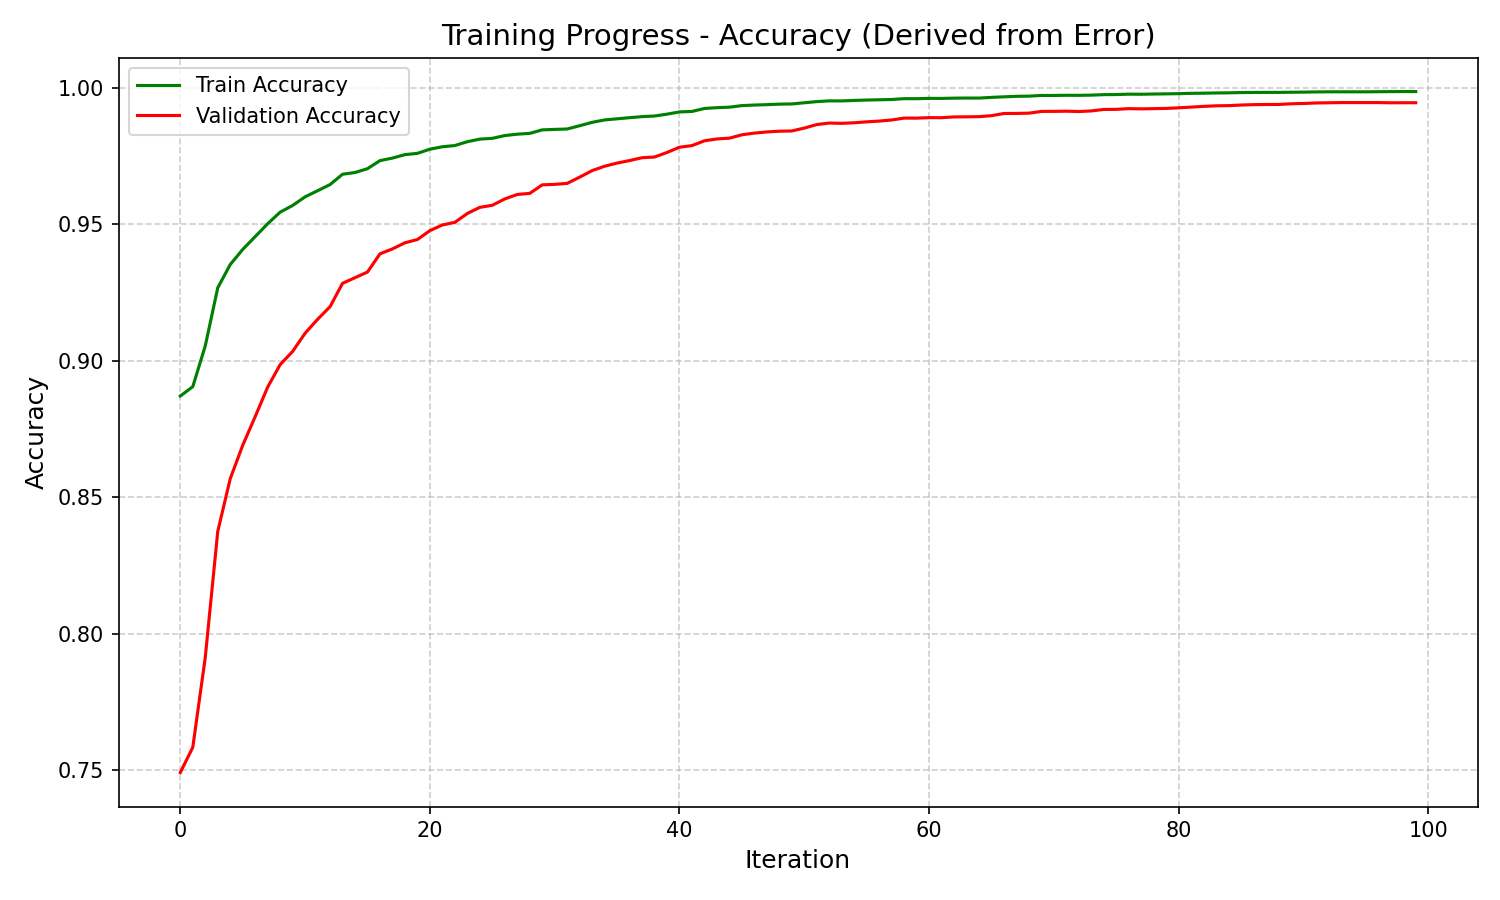
\includegraphics[width=\textwidth]{training_progress_accuracy.png}
    \caption{Training Progress: Accuracy (Train vs Validation).}
    \label{fig:training_progress_accuracy}
\end{figure}


\subsubsection{Error Reduction}
\noindent
Figure~\ref{fig:training_progress_error} shows the error rate progression for both training and validation sets. The training error quickly reduces to near zero, while the validation error also decreases significantly, stabilizing at very low levels. This trend confirms the model's robustness and capacity for generalization.

\begin{figure}[H]
    \centering
    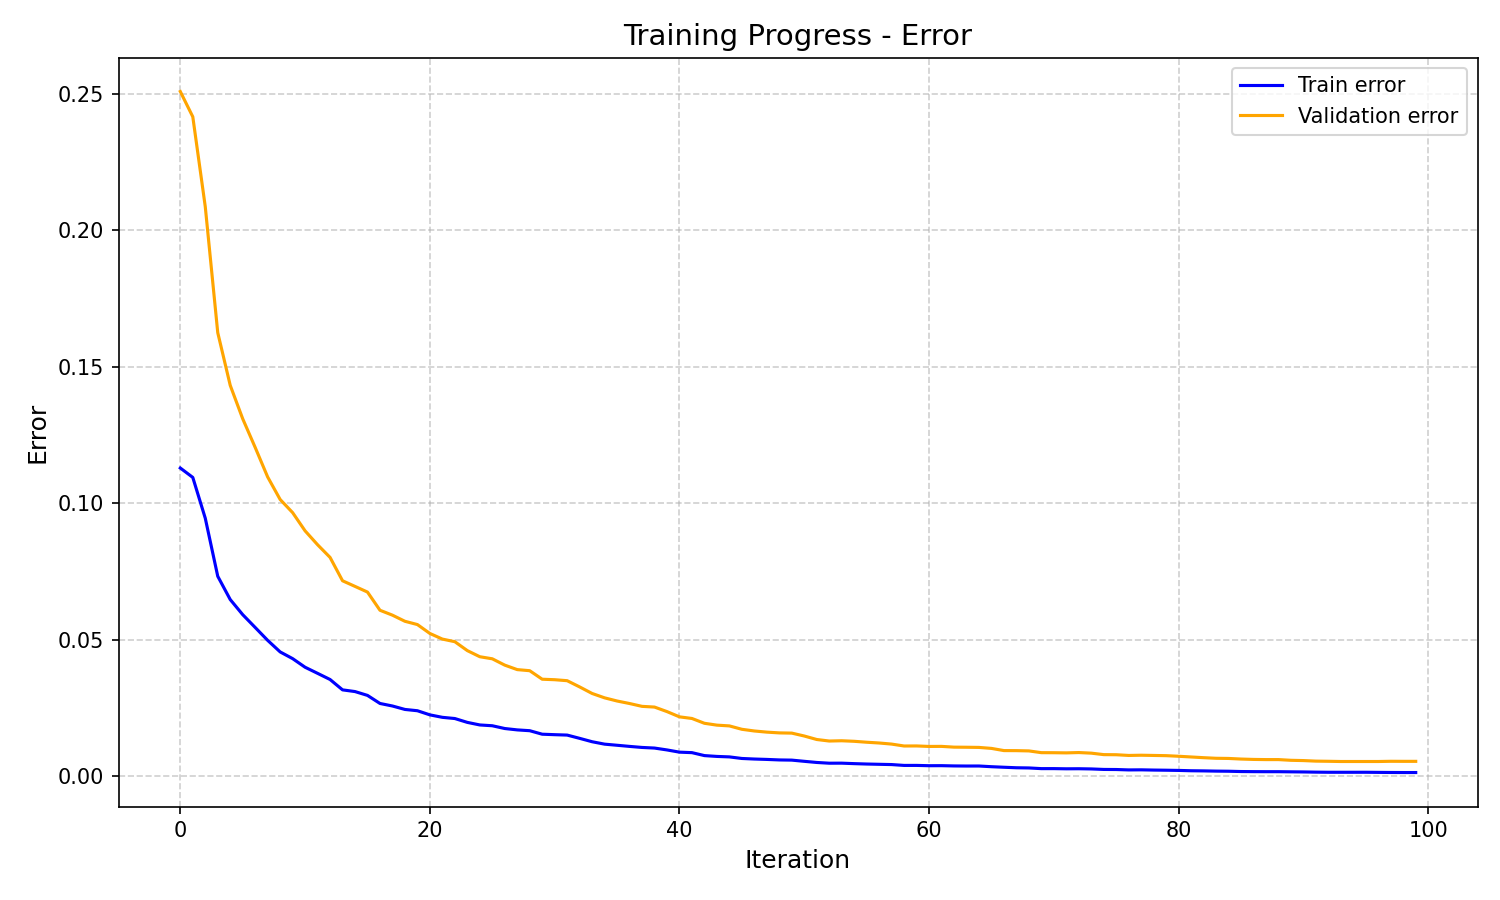
\includegraphics[width=\textwidth]{training_progress_error.png}
    \caption{Training Progress: Error Rate (Train vs Validation).}
    \label{fig:training_progress_error}
\end{figure}

\subsubsection{Log-Loss Convergence}
\noindent
Log-loss, a measure of prediction confidence, steadily decreases for both training and validation datasets, as depicted in Figure~\ref{fig:training_progress_logloss}. Validation log-loss stabilizes around 0.023, signifying high confidence in predictions and consistent model performance.

\begin{figure}[H]
    \centering
    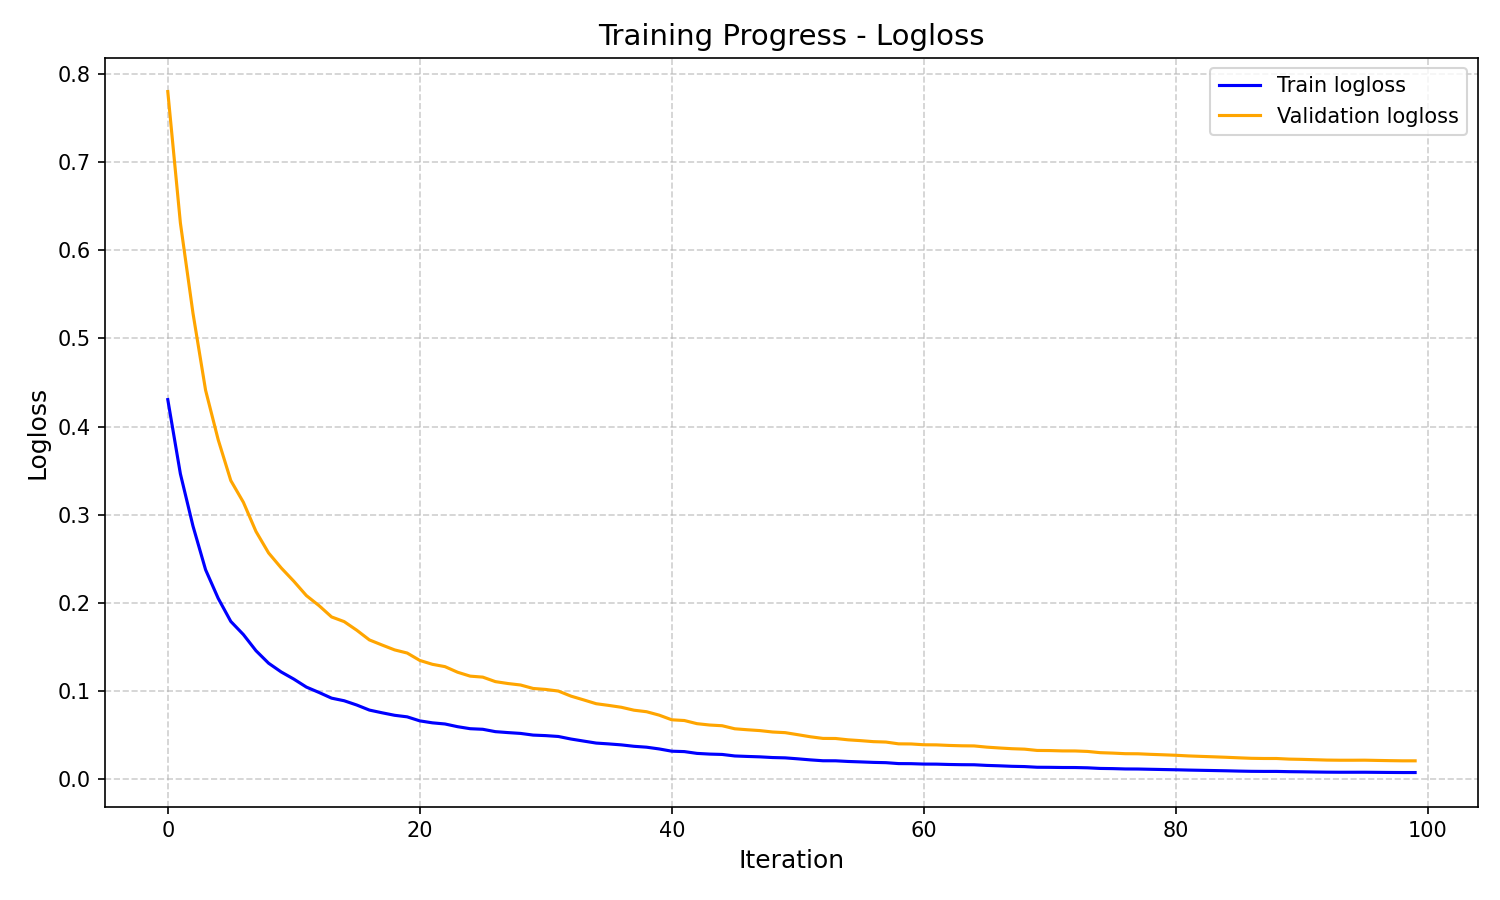
\includegraphics[width=\textwidth]{training_progress_logloss.png}
    \caption{Training Progress: Log-Loss (Train vs Validation).}
    \label{fig:training_progress_logloss}
\end{figure}

Across these figures, the minimal gap between training and validation metrics reflects strong
generalization—critical for real-world OSM data that can vary significantly by region or time.
These insights confirm that the final XGBoost model converges effectively, balancing low false
positives with a high capture rate for vandalism edits. When combined with the chunk-based data ingestion pipeline and carefully engineered features (\S\ref{sec:feature_construction}), this trained classifier forms
the linchpin of our vandalism detection system, ready to perform inference on live or monthly
OSM updates.


\newpage
\section{Enhancing Changeset-Level Detection}
\label{sec:changeset_level_detection}

In OpenStreetMap (OSM), a \emph{changeset} encapsulates a group of edits uploaded in one session, potentially spanning extensive geographic areas or multiple features. The same XGBoost pipeline discussed in previous sections can be trained on changeset-level data to detect vandalism for each session. However, additional techniques—the \emph{hyper-classifier} and \emph{meta-classifier}—provide further refinement by leveraging per-contribution predictions and fusing them with session-level insights.

\subsection{Baseline Changeset Pipeline}
\label{subsec:baseline_changeset_pipeline}

When operating on changeset data, the pipeline treats each \emph{changeset} as a single data instance, extracting session-level attributes (e.g., bounding-box extents, user metadata, and edit counts) as features. Although these features—discussed in Section~\ref{sec:feature_construction}—can capture large-scale vandalism (e.g., mass deletions), they may overlook subtle patterns of dispersed suspicious edits. An XGBoost classifier trained on these session-level attributes forms the baseline changeset approach.

\paragraph{High-Level Approach.}
\begin{enumerate}
    \item \textbf{Data Ingestion}: Load changeset-level records, each labeled as vandalism or non-vandalism.
    \item \textbf{Feature Extraction}: Incorporate bounding-box coordinates, timestamps, user statistics, and edit counts as input to the pipeline.
    \item \textbf{Training}: Fit an XGBoost model to classify each changeset, producing a vandalism probability per session.
\end{enumerate}

This baseline method effectively detects obvious session-wide disruptions (e.g., hundreds of deleted roads) but may miss more nuanced, distributed forms of vandalism if they lack a clear bounding-box or user-based signature.

\subsection{Hyper-Classifier: Aggregating Per-Contribution Predictions}
\label{subsec:hyper_classifier}

To overcome the limitations of purely changeset-level attributes, the pipeline incorporates the \emph{hyper-classifier}, which aggregates the output of the contribution-level XGBoost model. Rather than solely relying on bounding-box or changeset metadata, the hyper-classifier builds new features summarizing how suspicious each edit is within a session.

\paragraph{Aggregated Signals.}
\begin{enumerate}
    \item \textbf{Per-Contribution Probabilities}: For each edit, the contribution-level model outputs a vandalism probability (\texttt{pred\_prob}).
    \item \textbf{Group by Changeset}: All edits sharing a \texttt{changeset\_id} are collected, and their probabilities undergo statistical summarization (e.g., mean, median, quantiles, standard deviation, proportion of edits above a threshold).
    \item \textbf{Feature Matrix}: A new dataset emerges, where each row is a changeset, augmented with these aggregated per-edit probabilities.
    \item \textbf{Hyper-Classifier Training}: An additional XGBoost model is trained on this feature matrix to classify entire sessions, potentially capturing session-wide malicious intent that the baseline changeset pipeline might miss.
\end{enumerate}

\noindent
By consolidating the edit-level suspicion scores, the hyper-classifier aims to exceed the performance of the baseline session-level approach. The underlying assumption is that if many edits within a single changeset are moderately suspicious, the collective signal is significantly stronger than each edit’s individual suspicion.

\subsection{Meta-Classifier: Fusing Changeset-Level Base pipeline and Hyperclassifier Outputs}
\label{subsec:meta_classifier}

While the baseline changeset pipeline capitalizes on changeset metadata (bounding-box size, user stats, etc.), and the hyper-classifier exploits aggregated per-edit probabilities, each perspective covers different facets of vandalism. The \emph{meta-classifier} merges these two probability streams into a single final prediction. The motivation is to see if fusing these distinct probability streams yields better results than using either model alone.

\begin{enumerate}
    \item \textbf{Obtain Baseline Changeset Probability}: Run the session-level XGBoost model on changeset data, generating a vandalism probability.
    \item \textbf{Obtain Hyper-Classifier Probability}: Compute the probability that the same changeset is vandalism based on aggregated per-edit signals.
    \item \textbf{Construct a New Dataset}: Each changeset now has two predicted probabilities (\(\hat{p}_{\textnormal{session}}\) and \(\hat{p}_{\textnormal{hyper}}\)), along with a true label indicating whether it is vandalism.
    \item \textbf{Train Meta-Classifier}: A separate XGBoost or logistic regression model maps these two probabilities (and optionally a few additional features) to a final vandalism classification.
\end{enumerate}

\noindent
During inference, the pipeline once again obtains predictions from both the normal model and the hyper-classifier, feeding them into the meta-classifier to arrive at a single decision.

To facilitate the hyper-classifier and meta-classifier, changeset IDs must be consistent between datasets. If a changeset or its constituent edits are missing in the contribution-level data, they cannot be aggregated. Hence, both the hyper-classifier and meta-classifier pipelines require a matched set of edits and changesets.

\paragraph{Conclusion.}

The multi-stage approach to changeset-level detection (baseline pipeline, hyper-classifier, and meta-classifier) highlights the system’s flexibility. The baseline pipeline uses a straightforward session-level model, the hyper-classifier exploits fine-grained edit suspicions, and the meta-classifier fuses both perspectives. Although additional complexity is introduced, each stage addresses a different source of vandalism signals.

All three methods are independently trained using XGBoost. The pipeline organizes each stage’s training and evaluation data in alignment with the changeset splits outlined in Section~\ref{sec:data_splitting}, ensuring no data leakage between these overlapping models. Chapter~\ref{chapter:model_performance} provides empirical results, showing how these layered models can substantially improve detection accuracy across diverse OSM vandalism scenarios.


\section{Evaluation}
\label{sec:evaluation}

\subsection{Evaluation Metrics}
\label{sec:evaluation_metrics}

Measuring vandalism detection performance involves navigating a trade-off between false alarms and undetected malicious edits. The thesis employs a suite of metrics that highlight different facets of classification quality.

\paragraph{Precision, Recall, and F1-score.}
These metrics encapsulate distinct but complementary concerns:
\begin{itemize}
    \item \textbf{Precision}: Among the edits flagged as vandalism, how many are truly malicious?
    \item \textbf{Recall}: Of all vandalism edits in the dataset, how many did the model catch?
    \item \textbf{F1-score}: The harmonic mean of precision and recall, penalizing weaknesses in either dimension.
\end{itemize}
Because vandalism typically makes up a minority of OSM edits, achieving strong recall (to catch most malicious contributions) without overwhelming moderators with false positives is paramount.

\paragraph{AUC-PR vs. AUC-ROC.}
\noindent
When dealing with class imbalance, the area under the precision-recall curve (AUC-PR) can provide a clearer snapshot of performance than AUC-ROC. AUC-PR emphasizes how effectively the model maintains high recall while keeping false positives in check—a crucial balance in real-time vandalism detection. Nevertheless, the area under the receiver operating characteristic curve (AUC-ROC) remains valuable for a broader sense of discriminative power.

\noindent
Later sections present confusion matrices and curves (\autoref{fig:confusion_matrix}, \autoref{fig:precision_recall}, \autoref{fig:roc_curve}) that illustrate how these metrics play out in practice, demonstrating the classifier’s capacity to distinguish vandalism from normal edits.

\subsection{Bootstrapping for Confidence Intervals}
\label{sec:bootstrapping_for_ci}

While a single test set offers a snapshot of model performance, \textbf{bootstrapping} yields deeper insight into metric stability and variance. The procedure involves:
\begin{enumerate}
    \item \emph{Resampling} the test set with replacement multiple times (e.g., 1,000 iterations).
    \item \emph{Evaluating} metrics (precision, recall, F1-score, AUC-PR, etc.) for each resampled dataset.
    \item \emph{Aggregating} these results into distributions, computing mean, median, and confidence intervals.
\end{enumerate}
This Monte Carlo–style approach clarifies how sensitive the classifier is to the particular composition of the test set. Narrow intervals suggest a robust, reliable model, while wider bounds may indicate volatility in classification performance. Refer to \autoref{tab:bootstrap_metrics} for an example of how these confidence intervals provide a nuanced perspective on vandalism detection reliability.

\subsection{Geographical Evaluations}
\label{sec:geographical_evaluations}

OpenStreetMap (OSM) is a global resource, edited by contributors across diverse continents and countries. Because mapping practices, data availability, and local conventions can differ substantially from one region to another, a vandalism-detection model that excels in one geographical area may falter in another. To ensure broad applicability, we incorporate \emph{geographical evaluations}, systematically breaking down performance by region or continent.

In practice, this entails tagging each data instance—whether a single edit or an entire changeset—with the relevant continent or country. During post-processing, the model’s predictions are grouped by these spatial labels, and metrics such as precision, recall, and F1-score are recalculated within each group. If certain areas experience high error rates (e.g., a lower recall in Africa or an inflated false-positive rate in Asia), it can signal that the model’s learned patterns do not generalize effectively to those contexts. Explanations might include insufficient training samples from that region, differences in local tagging conventions, or a higher prevalence of certain map features that the classifier has not learned to handle.

Such an analysis also paves the way for region-specific remediation. If the classifier repeatedly underperforms in an underrepresented continent, it may be beneficial to supplement the training set with additional data from that area, refine certain features (e.g., bounding-box logic for roads in mountainous terrain), or even implement custom logic that triggers extra checks in regions with historically higher vandalism rates. Further, by mapping the model’s false positives and false negatives spatially, domain experts or OSM community volunteers can better prioritize manual validation and adopt targeted improvements. Although the final numeric results of these geographical evaluations appear later in the thesis, the methodological framework itself—spatial tagging and region-specific performance scoring—embeds seamlessly within the broader pipeline and provides crucial diagnostic feedback on regional biases or gaps in generalization.

\paragraph{Summary of Evaluation.}
By combining multifaceted evaluation metrics, and bootstrap-based statistical checks, the thesis ensures a comprehensive assessment of model generalization. In Chapter~\ref{chapter:model_performance}, we examine how these metrics translate into tangible results, highlighting precision-recall trade-offs, confusion matrices, and the stability revealed by bootstrapped confidence intervals, geographical evaluations.


\section{Summary and Method Integration}
\label{sec:method_summary_integration}

In sum, the methodological framework presented across this chapter unites a range of strategies to detect vandalism at multiple levels of granularity and to validate performance under realistic conditions. The pipeline begins by loading and cleaning raw OSM data (\S\ref{sec:data_sources_preprocessing} and \S\ref{sec:feature_construction}), ensuring that each edit or changeset has consistent, well-defined features capturing geometry, user history, tags, and other relevant attributes. From there, the main classification approach utilizes a finely tuned XGBoost model (\S\ref{sec:core_classification_model}) to learn which patterns correlate with malicious edits—a process guided by appropriate split strategies, robust evaluation metrics, and bootstrapping for confidence intervals.

Because vandalism can appear at different scales, the pipeline extends beyond per-contribution classification to changeset-level modeling, leveraging both a normal changeset model (built on session metadata) and a hyper-classifier (aggregating probabilities derived from individual edits). Finally, a meta-classifier can fuse the outputs of these changeset-level classifiers, capitalizing on the complementary nature of session metadata and aggregated per-contribution signals (\S\ref{sec:changeset_level_detection}).

The additional element described in this section—namely, geographical evaluations (\S\ref{sec:geographical_evaluations})—further enhance our capacity to diagnose and refine the system. By analyzing performance broken down by continent or country, the pipeline can highlight region-specific strengths or weaknesses, informing targeted improvements.

Taken together, these components illustrate a method that is both \emph{comprehensive}—covering local anomalies, aggregated session patterns, and large-scale evaluation—and \emph{flexible} in addressing multiple forms of vandalism. The next chapters will present empirical results demonstrating the effectiveness of this approach, accompanied by deeper discussions of how these methodological choices impact performance in real-world scenarios.


%---------------------------------------------
% Chapter 4: Model Performance
%---------------------------------------------
\chapter{Model Performance}
\label{chapter:model_performance}

This chapter presents a detailed evaluation of the machine learning models developed for vandalism detection in OpenStreetMap (OSM). Both contribution-level and changeset-level models are analyzed, focusing on their ability to generalize across diverse data splits, the robustness of their predictions, and the role of user and OSM element features (abbreviated as U, OE features) in enhancing detection capabilities.

\section{Contribution-Level Model Performance}
\label{sec:contribution_model_perf}

The contribution-level model operates at the granularity of individual edits, identifying malicious modifications before they aggregate into broader upload sessions. To comprehensively assess this model, we tested three distinct data split strategies:
\begin{itemize}
    \item \textbf{Random Split}: Random partitioning into training, validation, and test sets, using 42 as the random seed. The sizes were configured as \texttt{TEST\_SIZE} = 150,000, \texttt{VAL\_SIZE} = 50,000, and a remaining large training set.
    \item \textbf{Geographic Split (by Continent)}: Training on specified regions (Oceania, Europe, South America), validating on others (Africa, Antarctica, Other), and testing on North America/Asia. The split key was \texttt{'continent'}, reflecting real-world geographic variability.
    \item \textbf{Temporal Split}: Training on 2018--2019 data, validating on 2015, and testing on 2017 (\texttt{TRAIN\_YEARS}, \texttt{VAL\_YEARS}, \texttt{TEST\_YEARS}), thus evaluating how well the model generalizes to later edits.
\end{itemize}

The following sections compare the model’s performance under these scenarios, with and without U, OE features.

\subsection{Model Performance Across Split Types}
\label{sec:split_performance}

Table~\ref{tab:vandalism_detection_final_clean} summarizes the performance metrics across random, geographic, and temporal splits. These metrics include \emph{Accuracy}, \emph{Precision}, \emph{Recall}, \emph{F1 score}, \emph{AUC-PR}, and \emph{ROC-AUC}. Each row indicates whether user and OSM element features are enabled.

\begin{table}[h!]
    \centering
    \renewcommand{\arraystretch}{2.5} % Increase row spacing for tables
    \captionsetup{font=small, labelfont=bf} % Caption settings
    \caption{Vandalism detection performance for different data split types regarding accuracy, precision, recall, F1 score, AUC-PR, and ROC-AUC [\%]. \vspace{0.3cm} \newline Note: U, OE features: User and OSM Element features}
    \vspace{1cm}
    \label{tab:vandalism_detection_final_clean}
    \resizebox{\textwidth}{!}{%
    \begin{tabular}{
        |l||l| ccccc c|
    }
    \hline
    \textbf{Data split type} & \textbf{Model type} & \textbf{Accuracy} & \textbf{Precision} & \textbf{Recall} & \textbf{F1 score} & \textbf{AUC-PR Score} & \textbf{ROC-AUC} \\
    \hline\hline
    \multirow{2}{*}{\textbf{Random Split}}
     & With U, OE features & \textbf{0.9931} & \textbf{0.9673} & \textbf{0.9994} & \textbf{0.9831} & \textbf{0.99969} & \textbf{0.99991} \\
     & Without U, OE features & 0.9742 & 0.8868 & 0.9986 & 0.9394 & 0.99742 & 0.99936 \\
    \cdashline{1-8}[0.8pt/2pt]
    \multirow{2}{*}{\textbf{Geo Split}}
     & With U, OE features & \textbf{0.8063} & \textbf{0.7818} & 0.7706 & \textbf{0.7762} & \textbf{0.87210} & \textbf{0.91040} \\
     & Without U, OE features & 0.5702 & 0.5155 & \textbf{0.9884} & 0.6776 & 0.61682 & 0.63373 \\
    \cdashline{1-8}[0.8pt/2pt]
    \multirow{2}{*}{\textbf{Temporal Split}}
     & With U, OE features & \textbf{0.7213} & \textbf{0.7460} & \textbf{0.8379} & \textbf{0.7893} & \textbf{0.85336} & 0.79453 \\
     & Without U, OE features & 0.7093 & 0.7106 & 0.7968 & 0.7512 & 0.83770 & \textbf{0.80316} \\
     \hline
    \end{tabular}
    }
\end{table}

\paragraph{Random Split:}
This configuration treats the entire dataset uniformly, distributing samples randomly into train, validation, and test partitions. With U, OE features, the model achieves high accuracy (99.31\%) and AUC-PR (99.969\%), reflecting a robust ability to identify vandalism. Recall is notably strong at 99.94\%, ensuring minimal missed vandalism. When these features are disabled, accuracy decreases to 97.42\%, indicating that user and OSM element attributes are critical for capturing nuanced vandalism behaviors.

\paragraph{Geographical Split:}
In this setup, training occurs on some continents while validation and testing occur on distinct regions. While the with-U, OE model attains a decent accuracy of 80.63\%, it underscores the challenges of regional variability, especially compared to the random split. The performance drop when excluding U, OE features (accuracy plunging to 57.02\%) suggests that user behavior and local OSM element patterns are pivotal for handling cross-region data differences.

\paragraph{Temporal Split:}
Here, older data (e.g., 2018--2019) trains the model, while newer edits (e.g., 2017 or other designated test year) form the test set. Accuracy (72.13\%) and recall (83.79\%) remain decent with U, OE features, highlighting the model’s ability to adapt over time, though not as strongly as under random conditions. Removing U, OE features diminishes performance further, revealing the difficulty of extrapolating older user behavior into newer vandalism patterns without comprehensive historical signals.

\paragraph{Observations and Significance:}
Across all split types, user and OSM element features consistently bolster metrics—most strikingly in geographical splits. Varying data distributions (regional or temporal) amplify the model’s need for contextual signals, underscoring user-level editing traits and OSM geometry changes as essential components in detecting and understanding vandalism. These findings guide subsequent steps in evaluating our best model configurations in greater detail.

\subsection{Visualizing Metrics for the Best Model}
\label{sec:visualizing_metrics}

This subsection focuses on the best-performing configuration—namely, the \emph{random split} combined with user and OSM element (U, OE) features. By presenting and interpreting key visualizations, we aim to provide deeper insights into the model’s classification strengths and limitations.

\paragraph{Confusion Matrix.}
Figure~\ref{fig:confusion_matrix} shows the distribution of true positives (TP), true negatives (TN), false positives (FP), and false negatives (FN) for vandalism detection. Numerically, the model correctly identifies the majority of non-vandalism contributions (TN) and vandalism contributions (TP), while maintaining a minimal fraction of misclassifications (FP and FN). This balance is critical for OSM workflows, as excessive FP can overwhelm human reviewers, while excessive FN risks undetected malicious edits.

\begin{figure}[H]
    \centering
    \includegraphics[width=0.8\textwidth]{confusion_matrix.png}
    \caption{Confusion matrix for the best-performing model (random split with U, OE features).}
    \label{fig:confusion_matrix}
\end{figure}

\paragraph{Precision-Recall Curve.}
In vandalism detection, vandalism contributions typically form the minority class. Figure~\ref{fig:precision_recall} plots precision versus recall across varying classification thresholds, highlighting how effectively the model minimizes false positives (maintains high precision) while capturing the majority of true vandalism edits (high recall). The near-ideal curve indicates that precision remains high across a wide range of recall levels—a crucial property when balancing the cost of manual review versus missed vandalism incidents.

\begin{figure}[H]
    \centering
    \includegraphics[width=0.8\textwidth]{precision_recall_curve.png}
    \caption{Precision-recall curve for the best-performing contribution-level model.}
    \label{fig:precision_recall}
\end{figure}

\paragraph{ROC Curve.}
The receiver operating characteristic (ROC) curve in Figure~\ref{fig:roc_curve} illustrates the relationship between the true positive rate (TPR) and false positive rate (FPR). This best model closely hugs the top-left corner, yielding an AUC near 1.0—a strong indicator that the model consistently distinguishes vandalism from legitimate contributions without inflating FPR. Such performance is pivotal for OSM’s large-scale environment, where even a small misclassification rate can translate into numerous erroneous flags or undetected vandal edits.

\begin{figure}[H]
    \centering
    \includegraphics[width=0.8\textwidth]{roc_curve.png}
    \caption{ROC curve for the best-performing contribution-level model.}
    \label{fig:roc_curve}
\end{figure}

\paragraph{Overall Observations.}
These visualizations reinforce the conclusions drawn from the quantitative metrics:
\begin{itemize}
    \item \textbf{Robust Classification}: The confusion matrix reveals very few misclassifications, implying minimal risk of undetected vandalism or unnecessary alerts.
    \item \textbf{Minority Class Excellence}: High precision-recall performance confirms that the model excels at flagging vandalism without overwhelming moderators with false positives.
    \item \textbf{Stable Threshold Behavior}: Both PR and ROC curves remain favorable across a wide range of thresholds, indicating stability and flexibility in real-world scenarios where decision boundaries may shift.
\end{itemize}

These findings underscore the importance of incorporating user and OSM element features into the detection pipeline, as they substantially enhance the model’s ability to capture subtle vandalism signals. The next section explores the robustness of these performance metrics through bootstrapping, providing confidence intervals to gauge variance in model predictions.

\subsection{Bootstrap Results for the Best Model}
\label{sec:bootstrap_best_model}

While the evaluation metrics in Section~\ref{sec:visualizing_metrics} highlight the strong performance of the model on a fixed test set, it is equally important to assess the \emph{stability} of these metrics under repeated sampling. Bootstrapping provides a robust mechanism for estimating variance and constructing confidence intervals, thereby revealing how sensitive the model is to variations in the test data.

\paragraph{Experimental Setup.}
The bootstrapping procedure involved drawing 1{,}000 random samples (with replacement) from the test set. Each sample maintained the same number of observations as the original test set, and the model’s metrics (Accuracy, Precision, Recall, F1-score, AUC-ROC, and AUC-PR) were computed for each iteration. Table~\ref{tab:bootstrap_metrics} presents the aggregated statistics over the 1{,}000 bootstrap iterations, providing insight into the mean, standard deviation, and 95\% confidence intervals for each metric.

\begin{table}[H]
    \centering
    \caption{Bootstrap Metrics (1,000 Iterations) for the Best Contribution-Level Model (Random Split with U/O Features).}
    \vspace{1cm}
    \label{tab:bootstrap_metrics}
    \renewcommand{\arraystretch}{1.3}
    {%
    \begin{tabular}{|l||r r r r|}
    \hline
    \textbf{Metric} & \textbf{Mean} & \textbf{Std Dev} & \textbf{95\% CI Lower} & \textbf{95\% CI Upper} \\
    \hline\hline
    Accuracy  & 0.99313 & 0.00022 & 0.99270 & 0.99357 \\
    \cdashline{1-5}[0.8pt/2pt]
    Precision & 0.96733 & 0.00105 & 0.96527 & 0.96941 \\
    \cdashline{1-5}[0.8pt/2pt]
    Recall    & 0.99943 & 0.00014 & 0.99914 & 0.99967 \\
    \cdashline{1-5}[0.8pt/2pt]
    F1-Score  & 0.98312 & 0.00054 & 0.98203 & 0.98418 \\
    \cdashline{1-5}[0.8pt/2pt]
    AUC-ROC   & 0.99992 & 0.00001 & 0.99989 & 0.99994 \\
    \cdashline{1-5}[0.8pt/2pt]
    AUC-PR    & 0.99970 & 0.00003 & 0.99963 & 0.99976 \\
    \hline
    \end{tabular}%
    }
\end{table}


\paragraph{Interpretation of Bootstrap Statistics.}
These bootstrap-derived statistics offer several key insights into model reliability:

\begin{itemize}
    \item \textbf{Consistency of Accuracy}: The mean accuracy of 0.99313, coupled with a low standard deviation (0.00022), suggests the model consistently maintains correct classification above 99\% of the time.
    \item \textbf{Precision Stability}: A mean precision of 0.96733 with tight confidence bounds (0.96527--0.96941) implies minimal fluctuation in false positives. This stability is crucial for real-world usage, where false alarms can burden moderators.
    \item \textbf{High Recall across Samples}: Recall remains exceptionally high at 0.99943, indicating that the model almost never misses vandalism, regardless of which subset of the test set is sampled.
    \item \textbf{Robust F1-Score}: The F1-score hovers around 0.983, reflecting a strong balance between precision and recall.
    \item \textbf{Near-Perfect AUC Metrics}: Both AUC-ROC (0.99992) and AUC-PR (0.99970) underscore the model’s powerful discriminative capabilities, with confidence intervals confined to a very narrow range.
\end{itemize}

\noindent The bootstrap analysis confirms that the high performance reported in Section~\ref{sec:visualizing_metrics} is not an artifact of a particular test split. Rather, the model maintains robust accuracy and class-specific metrics across repeated subsampling. This consistency highlights the effectiveness of incorporating user and OSM element features, reinforcing the conclusion that these feature sets are integral to robust vandalism detection. It also suggests that the model can be trusted to deliver stable results in production-like scenarios, where incoming edits may slightly differ from those observed in the test set.

\subsection{Geographical Evaluation Results for the Best Model}
\label{sec:geo_eval_best_model}

This subsection presents a continent-wise evaluation of our best-performing model, illustrating how well it adapts to regional variations in OpenStreetMap (OSM) vandalism. Table~\ref{tab:geo_eval_continents} summarizes key metrics (accuracy, precision, recall, F1-score, AUC-ROC, AUC-PR) across eight continent categories in the dataset, revealing consistently high performance with minor discrepancies attributed to data distribution and sample sizes.

\begin{table}[htbp]
    \centering
    \caption{Continent-Wise Metrics for the Best Model}
    \label{tab:geo_eval_metrics}
    \resizebox{\textwidth}{!}{
    \begin{tabular}{lrrrrr}
    \toprule
    \textbf{Continent} & \textbf{Accuracy} & \textbf{Precision} & \textbf{Recall} & \textbf{F1-Score} & \textbf{AUC-ROC} \\
    \midrule
    Africa         & 0.9973 & 0.9861 & 0.9998 & 0.9929 & 0.99999 \\
    Antarctica     & 1.0000 & 1.0000 & 1.0000 & 1.0000 & 1.00000 \\
    Asia           & 0.9927 & 0.9474 & 0.9990 & 0.9725 & 0.99993 \\
    Europe         & 0.9918 & 0.9601 & 0.9989 & 0.9791 & 0.99987 \\
    North America  & 0.9923 & 0.9623 & 1.0000 & 0.9808 & 0.99987 \\
    Oceania        & 0.9939 & 0.9835 & 0.9992 & 0.9913 & 0.99987 \\
    Other          & 0.9968 & 0.9904 & 1.0000 & 0.9952 & 0.99999 \\
    South America  & 0.9891 & 0.9672 & 0.9996 & 0.9831 & 0.99994 \\
    \bottomrule
    \end{tabular}
    }
\end{table}


\noindent
\textbf{Observations and Insights.}
\begin{itemize}
    \item \textbf{Overall High Accuracy Across Continents:}
    Most regions display above 98\% accuracy, underscoring the model’s robust generalization to different geographic contexts. Even South America, with the lowest accuracy of 98.91\%, remains close to the top end.

    \item \textbf{Near-Perfect Results in Antarctica:}
    Antarctica has only 23 samples, all classified correctly, yielding 100\% metrics. This perfect performance partly reflects the small sample size, making it easier to achieve flawless classification.

    \item \textbf{Minor Variation in Precision and Recall:}
    Precision hovers mostly above 96\%—indicating few false positives—and recall consistently nears 100\% in most continents, signifying that vandalism edits are rarely missed. Africa, for instance, shows a near-perfect recall of 0.9998, illustrating minimal undetected vandalism in that region’s dataset.

    \item \textbf{High AUC-ROC and AUC-PR Values:}
    All regions achieve AUC-ROC scores above 0.9998, revealing superior discrimination between vandalism and non-vandalism edits. In practice, this means the model selects a threshold that balances precision and recall effectively across diverse geographies.

    \item \textbf{Potential Influences of Data Distribution:}
    Africa, Asia, and Europe comprise large numbers of edits, offering the model abundant training examples. Regions like Antarctica or Oceania have fewer edits, which can lead to either perfect performance (e.g., Antarctica) or minor classification errors if the training distribution does not fully capture these areas’ editing patterns.

\end{itemize}

\noindent
These results validate the model’s capacity to handle global OSM edits, maintaining consistently high performance despite potential continental differences in editing style, user demographics, or map features. Although local factors (e.g., region-specific vandalism forms) could still pose challenges, the results suggest that the best model addresses the majority of vandalism scenarios around the world.

The next subsection (\S\ref{sec:importance_user_features}) delves deeper into why user and OSM element features bolster performance, comparing metrics between models with and without these features to illustrate their impact in a more nuanced manner.

\subsection{Importance of User and OSM Element Features}
\label{sec:importance_user_features}

User and OSM element (\textbf{U/O}) features have a pronounced effect on the model’s ability to distinguish malicious edits from legitimate contributions. This subsection provides both quantitative and qualitative insights into why these features matter, referencing comparative performance metrics, feature importance rankings, and domain-specific rationales.

\paragraph{Comparative Performance.}
Figure~\ref{fig:bar_graph_comparison} highlights how metrics such as precision, recall, F1-score, AUC-PR, and AUC-ROC increase significantly when U/O features are enabled compared to a baseline model that omits them. For instance, precision rises sharply due to the model’s enhanced capacity to identify truly vandalistic edits, minimizing spurious alerts. Similarly, recall improves, capturing more actual vandalism without sacrificing precision.

\begin{figure}[H]
    \centering
    \includegraphics[width=\textwidth]{bar_graph_comparision_pcuof_vs_nuof.png}
    \caption{Metric comparison for models with and without user and OSM element (U/O) features, demonstrating clear performance gains when U/O features are included.}
    \label{fig:bar_graph_comparison}
\end{figure}

\paragraph{Feature Importance.}
Beyond raw metrics, the XGBoost framework enables interpretability via feature importance scores. Figure~\ref{fig:feature_importance} shows the top 20 features ranked by total gain, revealing a dominant presence of U/O features. High-ranking user-centric attributes, such as \texttt{user\_n\_changesets\_cum} or \texttt{user\_previous\_edit\_timestamp}, highlight how user histories and editing patterns offer critical clues. OSM element attributes, like \texttt{n\_edits} (cumulative edits on an object) or \texttt{element\_previous\_edit\_timestamp}, capture the recency and frequency of map-object changes, effectively flagging suspicious edit bursts or back-and-forth modifications.

\begin{figure}[H]
    \centering
    \includegraphics[width=\textwidth]{feature_importance.png}
    \caption{Top 20 features by total gain in the XGBoost model. U/O features dominate the upper ranks, underscoring their value in vandalism detection.}
    \label{fig:feature_importance}
\end{figure}

\subsubsection{Comparative Analysis of Geo-Split Models}
\label{sec:geo_split_analysis}

To evaluate the importance of user and OSM element features, an experiment was conducted comparing two models: one with user and OSM element features and one without. The analysis leveraged geo-splits by training, validating, and testing the models on geographically distinct regions such as Asia, Africa, Europe, Oceania, North America, South America, Antarctica, and Other. The bootstrap metrics were collected across multiple valid combinations of train, test, and validation regions, and the results are presented in Figure~\ref{fig:geo_bootstrap_comparison}.

\begin{figure}[H]
    \centering
    \includegraphics[width=0.8\textwidth]{geo_boot_strap_comparison.png}
    \caption{Comparison of Bootstrap Performance Metrics (Geo-Split Models). The box plots compare the performance of models trained with and without user and OSM features across accuracy, precision, recall, and F1-score.}
    \label{fig:geo_bootstrap_comparison}
\end{figure}

From the box plot shown in Figure~\ref{fig:geo_bootstrap_comparison}, the following observations can be made regarding the performance of the two models:

\textbf{1. Accuracy:} The model with user and OSM features demonstrates a higher median accuracy, with most values clustering around 0.8. In contrast, the model without these features has a lower median accuracy, centered around 0.65. While the interquartile range is narrower for the model without features, the overall performance is less consistent and inferior.

\textbf{2. Precision:} The feature-rich model exhibits a higher median precision, indicating better performance in identifying relevant results. The precision for the model without user and OSM features is significantly lower, with a narrower spread, suggesting limited relevance detection.

\textbf{3. Recall:} The model with user and OSM features has a slightly lower median recall compared to its other metrics, but it still outperforms the feature-less model. The feature-less model shows a slightly higher recall but with significantly larger variability, implying inconsistent performance across different geo-splits.

\textbf{4. F1 Score:} The model with user and OSM features maintains a higher median F1 score, reflecting a better balance between precision and recall. The feature-less model has a noticeably lower F1 score, indicating a suboptimal trade-off between these metrics.

\textbf{Overall Insights:}
The results highlight the clear advantage of incorporating user and OSM element features into the model. These features improve performance across all metrics, with the most significant gains observed in precision and accuracy. While there is some overlap in recall performance, the feature-rich model remains more consistent. This analysis underscores the importance of user behavior and OSM metadata in capturing spatial and contextual nuances, ultimately enhancing the model's ability to detect vandalism effectively.



\paragraph{Discussion and Domain Rationale.}
The synergy between user and element features is particularly evident in complex vandalism scenarios. For example:
\begin{enumerate}
    \item \textbf{User Histories and Behavior Patterns}:
    Attributes such as \texttt{user\_n\_changesets\_cum} and \texttt{user\_n\_edit\_days\_cum} reveal long-term behavioral trends. A contributor who shows abnormally high activity in a short span or a history of contentious edits is more likely to commit vandalism. Thus, user-based metrics add a layer of personalized detection that purely content-based features might miss.

    \item \textbf{OSM Element Details}:
    Indicators like \texttt{n\_edits} for a specific road or building denote how frequently the object has been changed. A series of rapid, repetitive edits on the same element may signal disputes, edit wars, or back-and-forth vandalism. By tying suspicious activity to the element level, the model pinpoints hot spots in the map.

    \item \textbf{Spatial/Temporal Contexts}:
    Combining user and element signals with geometry and timestamps further refines predictions. For instance, a user who rarely edits outside a specific region but suddenly modifies data in a distant locale may trigger a higher vandalism likelihood. Similarly, temporal features (\texttt{user\_time\_since\_previous\_edit}) help detect bursts of edits that deviate from normal user patterns.

    \item \textbf{Robustness Across Splits}:
    As evidenced in Table~\ref{tab:vandalism_detection_final_clean}, models with U/O features exhibit consistent gains under random, geographic, and temporal splits. By capturing both who is editing and what is being edited, the model generalizes better to unseen regions or future data.
\end{enumerate}

\noindent
These observations explain the metrics gap between models with and without U/O features. In essence, user features highlight contributor credibility and patterns, while element features enable a fine-grained view of object-based anomalies. Their combined effect sustains high precision and recall across various data splits, rendering the detection pipeline significantly more robust against the diverse forms of vandalism encountered in OSM.


\section{Changeset-Level Model Performance}
\label{sec:changeset_level_performance}

This section evaluates three approaches for vandalism detection at the \emph{changeset} level:
\begin{enumerate*}
    \item A \textbf{baseline XGBoost model} (trained on changeset-level features \S\ref{sec:features_changeset}),
    \item The \textbf{hyper-classifier} (incorporating aggregated per-contribution signals), and
    \item The \textbf{meta-classifier} (fusing outputs from the first two models).
\end{enumerate*}

\vspace{0.5em}
\noindent As discussed in Section~\ref{sec:changeset_level_detection}, each model addresses session-wide vandalism from a different angle; the hyper-classifier leverages micro-level signals by aggregating suspicious edits, whereas the baseline model focuses on direct changeset attributes, and the meta-classifier attempts to unify both.


\subsection{Overview of Model Results}

Table~\ref{tab:changeset_comparison} summarizes the performance of the three models in terms of accuracy, precision, recall, F1-score, and AUC-ROC. Notably, while the baseline model offers moderate performance, the hyper-classifier yields significantly higher metrics. The meta-classifier, in this dataset, does not surpass the hyper-classifier, indicating that aggregating contribution-level probabilities already captures most session-level signals.

\begin{table}[htbp]
    \centering
    \caption{Comparison of Changeset-Level Models}
    \label{tab:changeset_comparison}
    \begin{tabular}{lccccc}
    \toprule
    \textbf{Model} & \textbf{Accuracy} & \textbf{Precision} & \textbf{Recall} & \textbf{F1-Score} & \textbf{AUC-ROC}\\
    \midrule
    Baseline XGBoost (Changeset) & 0.8715 & 0.8713 & 0.8773 & 0.8743 & 0.9440 \\
    Hyper-Classifier             & 0.9761 & 0.9806 & 0.9724 & 0.9765 & 0.9962 \\
    Meta-Classifier              & 0.9744 & 0.9758 & 0.9739 & 0.9749 & 0.9961 \\
    \bottomrule
    \end{tabular}
\end{table}

\noindent
\textbf{Baseline XGBoost (Changeset):}
Attains approximately 87\% accuracy and F1-score, highlighting its competence in identifying large-scale vandalism from high-level changeset features. However, an AUC-ROC of 0.9440 indicates it may struggle to cleanly separate malicious sessions from benign ones, especially when vandalism is subtle or distributed across numerous edits.

\noindent
\textbf{Hyper-Classifier:}
Aggregating suspicious-edit probabilities into changeset-level metrics drastically improves performance, reaching roughly 97.61\% accuracy with precision of 0.9806 and recall of 0.9724. This leap underscores the value of micro-level insights—if many edits in a session appear suspicious, the entire changeset is likely vandalistic. With an AUC-ROC of 0.9962, it convincingly differentiates harmful sessions from standard editing behavior.

\noindent
\textbf{Meta-Classifier:}
By merging the baseline changeset model’s probability with the hyper-classifier’s output, one might expect further gains. Here, however, the meta-classifier (0.9744 accuracy, 0.9961 AUC-ROC) does not exceed the hyper-classifier alone. This plateau suggests two possible factors:
\begin{itemize}
    \item The aggregated per-edit probabilities capture the majority of relevant information, leaving minimal unexplained variance for changeset-level features to exploit.
    \item Additional hyperparameter tuning for the meta-classifier (e.g., adjusting regularization, tree depth) may be needed to unlock any residual improvements.
\end{itemize}

\subsection{Discussion and Observations}

\begin{itemize}
    \item \textbf{Value of Per-Edit Aggregation}:
    The hyper-classifier’s strong performance highlights that modeling the distribution of suspicious edits within a changeset can substantially bolster detection accuracy. Even if single edits do not appear glaringly malicious, their collective pattern can signal high-risk sessions.
    \item \textbf{Meta-Classifier Plateau}:
    Although fusing both perspectives appears intuitively beneficial, our results indicate only marginal or no improvement over the hyper-classifier’s already-high performance. This outcome likely reflects the hyper-classifier’s ability to integrate most session-level cues implicitly, as well as the need for more extensive tuning of the meta-classifier to capitalize on potential synergies.
    \item \textbf{Real-World Implications}:
    For applications prioritizing precision and recall at the changeset level, adopting the hyper-classifier pipeline promises significant gains. The meta-classifier framework remains valuable if additional session features or refined training procedures reveal further performance potential.
\end{itemize}

Overall, the hyper-classifier stands out as the most effective changeset-level model in these experiments, demonstrating that aggregated per-contribution probabilities can reveal large-scale or distributed vandalism patterns. The meta-classifier’s performance indicates no immediate gains beyond the hyper-classifier, yet future iterations involving more extensive hyperparameter optimization or enriched changeset attributes may unlock further improvements.


%-------------------------------------------------
% CHAPTER: Application: Vandalism in OpenStreetMap
%-------------------------------------------------

\chapter{Application: Vandalism in OpenStreetMap} \label{chapter:application}

This chapter presents an analysis of the application of the proposed vandalism detection model on over two years of real-time OpenStreetMap (OSM) contributions (from January 2022 to July 2024). Using the prediction results, we evaluate temporal trends, highlight significant deviations, and discuss the implications for identifying and mitigating vandalism in OSM contributions.

\section{Overview of Vandalism Predictions}
The analysis covers monthly contributions and corresponding vandalism predictions over the study period. Predictions are based on the model's application to real-time datasets, enabling continuous monitoring of contributions for potential vandalism. Figures \ref{fig:vandalism_bar_graph} and \ref{fig:vandalism_line_graph} illustrate these trends using bar and line graphs, respectively.

\section{Key Observations and Analysis}

\subsection{General Trends}
Over the study period, OSM saw significant variation in monthly contributions, ranging from approximately \textbf{19 million} (July 2024) to \textbf{39 million} (August 2023). Vandalism counts exhibited similar variability, with predictions ranging from around \textbf{46,000} (December 2023) to a peak of over \textbf{1.3 million} (August 2023). These figures highlight a mix of stable months and periods of sudden spikes in vandalism, as seen in Figures \ref{fig:vandalism_bar_graph} and \ref{fig:vandalism_line_graph}.

\subsection{Deviations and Notable Outliers}
\textbf{August 2023 Spike:} The model flagged a dramatic increase in vandalism predictions, reaching over \textbf{1.3 million} entries, far exceeding the monthly average (Figure \ref{fig:vandalism_bar_graph}). This spike may be attributed to coordinated malicious activities or errors in contribution uploads. Notably, contributions also peaked at 39 million during this month, suggesting heightened activity.

\textbf{July 2023 Increase:} Another substantial increase in vandalism predictions (over \textbf{207,000} entries) aligns with a high number of contributions for that month (\textbf{24.7 million}). While less extreme than August, this warrants further investigation to determine whether user behavior changes or systemic factors were responsible.

\textbf{Temporal Stability in Early 2024:} From January to July 2024, vandalism counts appeared relatively stable, ranging between \textbf{49,000 and 72,000} predictions per month. This stability may reflect improved moderation or reduced malicious activity during this period.

\subsection{Seasonal Variability}
Seasonal patterns suggest that vandalism may fluctuate based on user activity trends. For instance, higher vandalism predictions often coincided with months of elevated contributions (Figure \ref{fig:vandalism_line_graph}), while periods like late 2022 and early 2023 exhibited comparatively lower vandalism rates.

\section{Implications for Real-Time Monitoring}
The insights gained from these predictions underscore the importance of implementing robust, scalable vandalism detection mechanisms in OSM. Key takeaways include:
\begin{itemize}
    \item \textbf{Spike Detection:} The ability to detect significant deviations (e.g., August 2023) provides an opportunity to investigate and address potential systemic issues or targeted vandalism campaigns.
    \item \textbf{Trend Analysis:} Regular monitoring of vandalism trends can help prioritize regions or periods for manual review by moderators, improving the overall quality of OSM contributions.
    \item \textbf{Scalability of the Model:} Despite the variability in contributions and vandalism counts, the model effectively scaled to handle datasets of varying sizes, demonstrating its practicality for large-scale applications.
\end{itemize}

\section{Visualizing Results}

\begin{figure}[H]
    \centering
    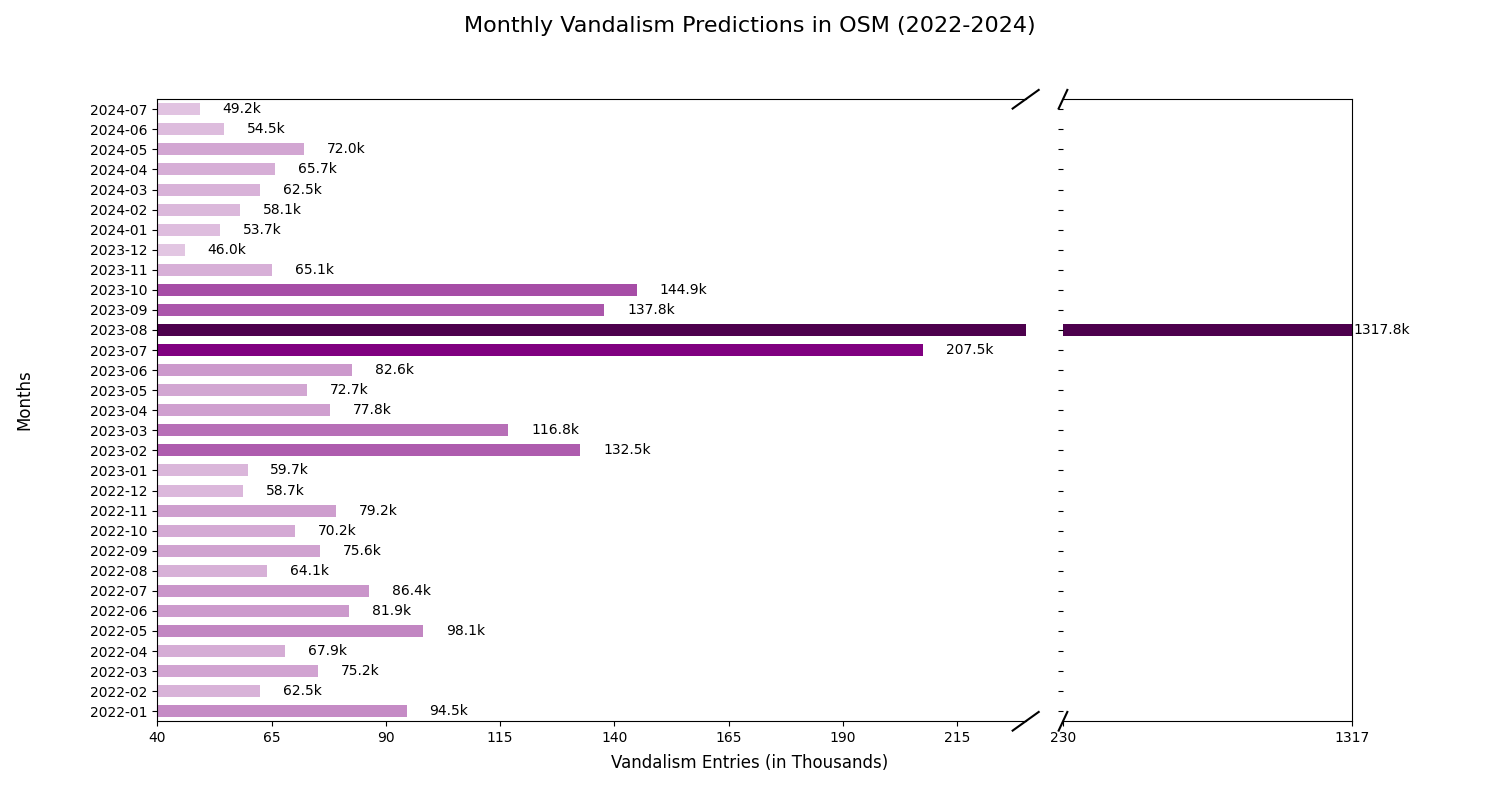
\includegraphics[width=\textwidth]{vandalism_predictions_2022_to_2024_bar_graph.png}
    \caption{Monthly vandalism predictions in OSM (2022–2024) – Bar Graph. The spike in August 2023 is evident, indicating a significant deviation from regular vandalism patterns.}
    \label{fig:vandalism_bar_graph}
\end{figure}

\begin{figure}[H]
    \centering
    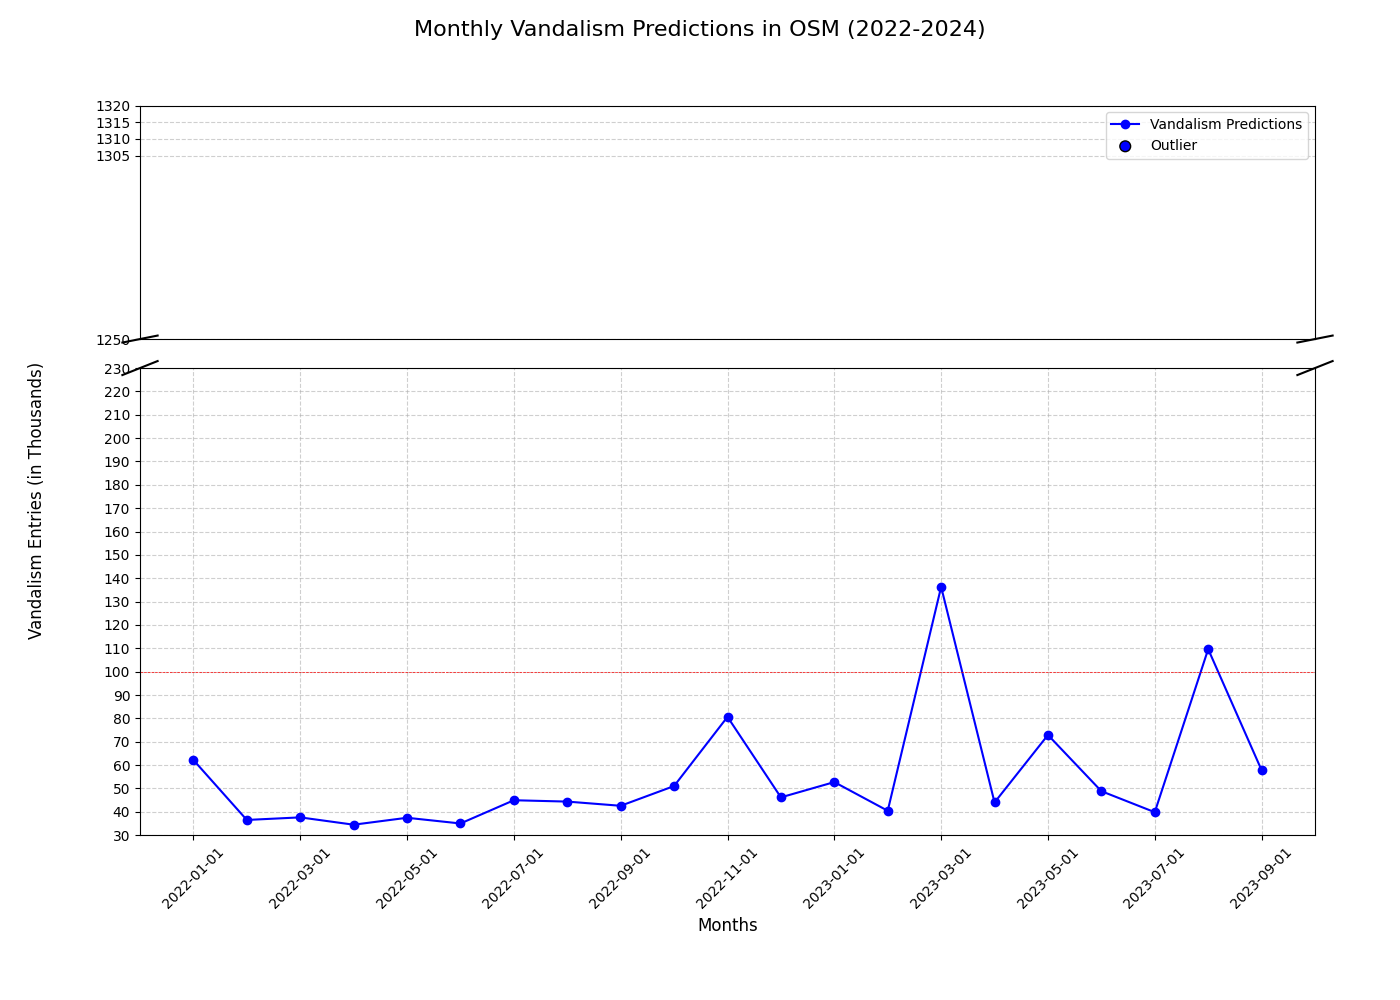
\includegraphics[width=\textwidth]{vandalism_predictions_2022_to_2024_line_graph.png}
    \caption{Monthly vandalism predictions in OSM (2022–2024) – Line Graph. Seasonal patterns and notable spikes, such as in August 2023, are highlighted.}
    \label{fig:vandalism_line_graph}
\end{figure}

\subsection{Heatmap Visualization}
To further understand the spatial distribution of vandalism, a heatmap was generated showing vandalism predictions across the world. The heatmap is available for interactive exploration, allowing users to visualize patterns for each month from January 2022 to July 2024. The static image in Figure \ref{fig:vandalism_heatmap_aug_2023} shows the distribution of vandalism for August 2023, where the spike in predictions aligns with regions experiencing heightened activity.

\noindent\textbf{Interactive Visualization:} The full heatmap can be accessed at the following link: \url{https://your-interactive-heatmap-link.com}

\begin{figure}[H]
    \centering
    \includegraphics[width=\textwidth]{vandalism_heat_map_aug_2023.png}
    \caption{Heatmap of vandalism predictions for August 2023. The spike in vandalism activity is prominently visible across highly active regions.}
    \label{fig:vandalism_heatmap_aug_2023}
\end{figure}


\section{Summary}
The application of the vandalism detection model to over two years of real-time data illustrates its effectiveness in identifying malicious contributions and its adaptability to dynamic OSM editing trends. While general predictions align with expected patterns, significant deviations (e.g., August 2023) highlight the need for continued refinement of detection systems and collaborative efforts to mitigate vandalism in OSM.

%---------------------------------------------
% Chapter 5: Discussions and Future Work
%---------------------------------------------
\chapter{Discussions and Future Work}
\label{chapter:discussions_and_future_work}

This chapter reflects on the key insights gained from implementing and evaluating the proposed vandalism detection framework, addressing the objectives and research questions put forth in Chapter~\ref{introduction}. In particular, it discusses the model’s practical integration into real-world OSM workflows, the importance of user and OSM element features, and the feasibility of scaling the approach to high-volume data streams. The chapter concludes with an outline of potential directions for future work to bolster the robustness and adaptability of this system.

\section{Discussion}
\label{sec:discussion}

\subsection{Achieving Robust Detection in Real-World Settings}
A primary ambition of this thesis was to train and validate the model on a moderately sized dataset (approximately 0.6 million labeled contributions) while ensuring that it generalizes effectively to real-time OSM edits. Preliminary real-world tests indicate that around 30 million new contributions may arrive monthly, underscoring the necessity of a pipeline that not only excels in predictive accuracy but also maintains rapid inference times.
\begin{itemize}
    \item \textbf{Prediction as a New Labeled Dataset:} The high precision and recall observed in Chapter~\ref{model_performance} suggest that model outputs can serve as a high-confidence labeled set, marking suspicious edits for manual review. This iterative process can continually refine the training corpus, thus improving the model over time.
    \item \textbf{Integration at HeiGIT:} Given the pipeline’s chunk-based architecture and proven scalability, it can be seamlessly linked to HeiGIT’s existing OSM data stream. The inference process (roughly 1.5 hours for monthly batch files) fits within the operational window of many data ingestion workflows, enabling near real-time identification of vandalism in 5-minute snapshots.
    \item \textbf{Inference Efficiency:} Despite the comprehensive set of features, including user histories and OSM element metadata, the final XGBoost classifier delivers swift predictions. This efficiency is pivotal in continuously monitoring OSM’s stream of edits, ensuring that flagged cases reach reviewers swiftly.
\end{itemize}

\subsection{Importance of User and OSM Element Features}
Chapters~\ref{model_performance} and \ref{background} jointly revealed that user-focused attributes (e.g., cumulative changesets, edit frequencies) and OSM element features (e.g., edit history on specific objects) significantly elevate the model’s capacity to spot vandalism. Empirical evidence shows:
\begin{itemize}
    \item \textbf{Better Geographical and Temporal Generalization:} Models enriched with user and element features performed more consistently under geographic (\S\ref{sec:geo_split_contrib}) and temporal splits (\S\ref{sec:temporal_split_contrib}), indicating that these signals capture enduring behavioral and object-based patterns less dependent on region or time.
    \item \textbf{Heightened Precision and Recall:} The metrics in Table~\ref{tab:vandalism_detection_final_clean} confirm large gains in precision and recall with these features enabled, particularly in high-variance settings. The boosted precision lowers false alarms, while higher recall ensures fewer malicious edits evade detection.
\end{itemize}
By integrating insights about who is editing and what is being edited, the model robustly identifies anomalous behaviors, even when novel forms of vandalism arise.

\subsection{Outcome Relative to Thesis Objectives and Research Questions}
The objectives introduced in Section~1.4 aimed to build a feature-rich, scalable ML pipeline capable of detecting vandalism with high accuracy while remaining computationally efficient. Key achievements include:
\begin{itemize}
    \item \textbf{Comprehensive Feature Engineering:} Spatial, temporal, user, and textual attributes were combined to capture the diversity of OSM data. Chapters~\ref{background} and \ref{model_performance} detailed how these features bolster accuracy in different split configurations.
    \item \textbf{Scalable ML Pipeline:} Chunk-based data loading and parallelized feature extraction allow the system to process millions of edits per month with minimal overhead. Inference times of roughly 1.5 hours for monthly data or real-time detection within a 5-minute window confirm operational viability.
    \item \textbf{High Predictive Performance:} The best XGBoost-based model attained precision and recall above 95\% in random splits, with robust performance in geographic and temporal splits as well. This aligns with the goal of minimizing false positives while maintaining strong detection of genuine vandalism.
    \item \textbf{User Behavior and Contextual Cues:} User-history features proved crucial for capturing recidivist or abrupt editing behaviors, while OSM element metadata flagged localized edit wars or repeated tampering. These findings address the research question of which signals most enhance vandalism detection.
\end{itemize}
Nonetheless, certain research questions persist around sustaining performance under evolving vandalism strategies and guaranteeing adaptation to newly emerging edit patterns.

\section{Future Work}
\label{sec:future_work}

Despite the demonstrated success, several avenues exist for further enhancement of the proposed system:

\begin{enumerate}
    \item \textbf{Real-Time Streaming and Continuous Learning:}
    While the current pipeline is chunk-based and efficient enough for monthly or near real-time data, an incremental or online learning framework could further reduce latency. This would allow immediate model updates in response to new edit behaviors or flagged vandalism cases.

    \item \textbf{Refined Data Labeling at Scale:}
    The thesis leverages a labeled dataset of around 0.6 million contributions. As predictions are integrated into OSM’s data stream at HeiGIT, an iterative feedback loop could generate more extensive, high-quality labels. Active learning or crowdsourced verification could refine class boundaries, especially for ambiguous edits.

    \item \textbf{Deep Learning Architectures and Transfer Learning:}
    While XGBoost proved optimal for tabular data, recent developments in transformer-based models (e.g., FT-Transformers) may yield benefits for extremely high-dimensional or sparse features. Future experiments can compare these architectures if data volumes justify the additional computational overhead.

    \item \textbf{Localized Models and Domain Adaptation:}
    Regional or city-level models might outperform a single global model, especially in highly specialized editing contexts. Domain adaptation techniques could further enhance cross-region or cross-time performance by reducing calibration overhead when shifting between geographies or time periods.

    \item \textbf{In-Depth Interpretability and Explanation:}
    While feature importances help unravel model decisions, advanced interpretability tools—such as SHAP (SHapley Additive exPlanations)—could clarify how each user-centric or OSM element attribute influences individual predictions. This granularity aids community trust and fosters collaborative improvement of detection rules.

\end{enumerate}

\noindent
By pursuing these directions, the vandalism detection pipeline can stay aligned with OSM’s ever-evolving landscape. Enhanced real-time responsiveness, larger labeled datasets, and advanced interpretability or domain adaptation would expand both the technical depth and practical utility of the framework.

\section{Conclusion}
In summary, the research has demonstrated the feasibility and effectiveness of a feature-rich, XGBoost-based pipeline to detect vandalism across diverse OSM editing patterns. The system's strong performance—further underscored by user and OSM element features—indicates a viable path toward large-scale, near real-time deployment. As OSM continues to grow and editing behaviors change, ongoing improvements to data labeling, model updating, and region-specific adaptation will be essential to sustain the high detection rates exhibited in this thesis.


\begin{thebibliography}{9}

\bibitem{osm_home}
\textit{OpenStreetMap}: \url{https://www.openstreetmap.org/}

\bibitem{vandalism_osm}
\textit{Vandalism in OSM}: \url{https://wiki.openstreetmap.org/wiki/Vandalism}

\bibitem{xgboost_documentation}
\textit{XGBoost Documentation}: \url{https://xgboost.readthedocs.io/en/stable/}

\bibitem{heigit_website}
\textit{Heidelberg Institute for Geoinformation Technology (HeiGIT)}: \url{https://heigit.org/}

\bibitem{osm_changesets}
\textit{Changeset in OSM}: \url{https://wiki.openstreetmap.org/wiki/Changeset}

\bibitem{Li2021}
Y. Li, J. Anderson, and Y. Niu,
\textit{Vandalism Detection in OpenStreetMap via User Embeddings},
Proceedings of the 30th ACM International Conference on Information and Knowledge Management, 2021. Available at: \url{https://dl.acm.org/doi/10.1145/3459637.3482213}.

\bibitem{Yuan2022}
Y. Yuan, J. Zhang, and S. Liu,
\textit{Attention-Based Vandalism Detection in OpenStreetMap},
arXiv preprint, 2022. Available at: \url{https://arxiv.org/abs/2201.10406}.

\bibitem{OSMPatrol}
M. Neis and A. Zipf,
\textit{OSMPatrol: A Framework for Detecting Malicious Edits in OpenStreetMap},
Proceedings of the AGILE Conference on Geographic Information Science, 2012. Available at: \url{https://agile-online.org/conference_paper/cds/agile_2012/proceedings/papers/252_shortpaper.pdf}.

\bibitem{OSMCha}
W. Almeida,
\textit{OSMCha: OpenStreetMap Changeset Analyzer},
2016. Available at: \url{https://osmcha.org/}.

\bibitem{Adler2010}
B. Adler, L. De Alfaro, and I. Pye,
\textit{Detecting Wikipedia vandalism using WikiTrust},
CLEF 2010.

\bibitem{Crescenzi2017}
V. Crescenzi, G. Mecca, and P. Merialdo,
\textit{Computational tools for Wikipedia vandalism detection},
Communications of the ACM, 2017.

\bibitem{Heindorf2016}
S. Heindorf, M. Potthast, G. Engels, and B. Stein,
\textit{Vandalism detection in Wikidata},
ACM International Conference on Information and Knowledge Management, 2017.

\bibitem{Heindorf2017}
S. Heindorf, M. Potthast, G. Engels, and B. Stein,
\textit{A comparative study of vandalism detection methods in collaborative knowledge bases},
ACM Transactions on Knowledge Discovery from Data, 2017.

\bibitem{Li2021}
Y. Li, J. Anderson, and Y. Niu,
\textit{Vandalism Detection in OpenStreetMap via User Embeddings},
Proceedings of the 30th ACM International Conference on Information and Knowledge Management (CIKM), 2021.

\bibitem{MartinezRico2019}
F. Martinez-Rico, J. C. Reyes-Ortiz, and L. G. Guerrero-Bonilla,
\textit{Deep learning for Wikipedia vandalism detection},
International Journal of Advanced Computer Science and Applications, 2019.

\bibitem{Neis2012}
P. Neis, M. Goetz, and A. Zipf,
\textit{Towards automatic vandalism detection in OpenStreetMap},
ISPRS International Journal of Geo-Information, 2012.

\bibitem{Truong2018}
Q. T. Truong, G. Touya, and C. de Runz,
\textit{Towards Vandalism Detection in OpenStreetMap Through a Data Driven Approach},
GIScience 2018.

\bibitem{Truong2020}
Q. T. Truong, G. Touya, and C. de Runz,
\textit{OSMWatchman: Learning How to Detect Vandalized Contributions in OSM Using a Random Forest Classifier},
ISPRS International Journal of Geo-Information, 2020.

\bibitem{Yuan2022}
Y. Yuan, J. Zhang, and S. Liu,
\textit{Attention-Based Vandalism Detection in OpenStreetMap},
arXiv preprint, 2022.

\bibitem{OSMPatrol}
P. Neis and A. Zipf,
\textit{OSMPatrol: A Tool for Monitoring and Repairing Vandalism in OpenStreetMap},
Proceedings of GIScience 2010.

\bibitem{OSMCha}
T. Schmitt, J. Anderson,
\textit{OSMCha: Detecting Anomalous Changes in OpenStreetMap Edits},
FOSS4G, 2018.

\bibitem{xgboost_paper}
T. Chen and C. Guestrin,
\textit{XGBoost: A Scalable Tree Boosting System},
Proceedings of the 22nd ACM SIGKDD International Conference on Knowledge Discovery and Data Mining, 2016.

\bibitem{Chen2016}
T. Chen and C. Guestrin,
\textit{XGBoost: A scalable tree boosting system},
Proceedings of the 22nd ACM SIGKDD International Conference on Knowledge Discovery and Data Mining, 2016.

\bibitem{Arik2021}
S. O. Arik and T. Pfister,
\textit{TabNet: Attentive interpretable tabular learning},
Proceedings of the AAAI Conference on Artificial Intelligence, 2021.

\bibitem{Gorishniy2021}
Y. Gorishniy, I. Rubachev, V. Khrulkov, and A. Babenko,
\textit{Revisiting deep learning models for tabular data},
Advances in Neural Information Processing Systems, 2021.

\bibitem{chen2016xgboost} T. Chen and C. Guestrin, "XGBoost: A Scalable Tree Boosting System," in \textit{Proceedings of the 22nd ACM SIGKDD International Conference on Knowledge Discovery and Data Mining}, 2016, pp. 785–794.

\bibitem{friedman2001greedy} J. H. Friedman, "Greedy Function Approximation: A Gradient Boosting Machine," \textit{Annals of Statistics}, vol. 29, no. 5, pp. 1189–1232, 2001.

\bibitem{tutorialspoint2025} Tutorialspoint, "XGBoost Architecture," Available at: \url{https://www.tutorialspoint.com/xgboost/xgboost-architecture.htm}, Accessed: January 2025.

\end{thebibliography}


\end{thebibliography}


\end{document}
